
% ==================================================
% เอกสารชี้แจงเกณฑ์การวัดและประเมินผลรายวิชาคณิตศาสตร์ ม.ปลาย (ยึดตามข้อความในภาพตรงๆ)
% ==================================================

\clearpage
\thispagestyle{empty} 

\begin{center}
	\begin{tcolorbox}[
		colback=cambridgeblue!15,
		colframe=cambridgeblue!50!black,
		boxrule=0.8pt,
		arc=2mm,
		width=\linewidth
		]
		\centering
		{\Large\bfseries โครงสร้างสัดส่วนคะแนนและการวัดผลประเมินผลรายวิชาคณิตศาสตร์}
	\end{tcolorbox}
\end{center}

\vspace{0.3cm}

\subsection*{รายละเอียดและเกณฑ์การเก็บคะแนน (Course Assessment Details)}

\vspace{0.2cm}

\begin{enumerate}[label=\arabic*)., leftmargin=2em, itemsep=0.8em]
	\item \textbf{ด้านความรู้ : สัดส่วน $40\%$}
	\begin{itemize}
		\item สอบประจำหน่วย : $10\%$
		\item สอบกลางภาค : $15\%$
		\item สอบปลายภาค : $15\%$
	\end{itemize}
	
	\vspace{0.1cm}
	\item \textbf{ด้านทักษะ/กระบวนการ : สัดส่วน $50\%$}
	\begin{itemize}
		\item สมุด/เอกสารประกอบการสอน/ใบกิจกรรม : $25\%$
		\item กิจกรรมรายบุคคล (ชิ้นงาน) : $5\%$
		\item กิจกรรมในชั้นเรียน : $10\%$
		\item Mind mapping : $10\%$
	\end{itemize}
	
	\vspace{0.1cm}
	\item \textbf{ด้านคุณลักษณะฯ : สัดส่วน $10\%$}
	\begin{itemize}
		\item ความตรงต่อเวลา : $3\%$
		\item เวลาเรียน (ขาด ลา มาสาย) : $3\%$
		\item การมีส่วนร่วมในชั้นเรียน : $4\%$
	\end{itemize}
\end{enumerate}

\newpage

\chapter{จำนวนจริง}
\section{จำนวนจริง}
จากหลักฐานที่ปรากฏ เชื่อกันว่ามนุษย์มีความคิดในเรื่องจำนวนมาตั้งแต่สมัยโบราณ สังเกตได้จากการบันทึกจำนวนสัตว์เลี้ยงโดยใช้ก้อนหินหรือรอยบากบนต้นไม้ ซึ่งเป็นการจับคู่หนึ่งต่อหนึ่งระหว่างสัตว์แต่ละตัวกับก้อนหินหรือรอยบาก เซตของจำนวนดังกล่าว เรียกว่า \textbf{เซตของจำนวนนับ} หรือ \textbf{เซตของจำนวนธรรมชาติ} ซึ่งเขียนแทนด้วย
\begin{equation*}
	\mathbb{N} = \{1, 2, 3, \ldots\}
\end{equation*}

เมื่อมีจำนวนนับขึ้นใช้แล้ว มนุษย์เริ่มใช้จำนวนในขอบข่ายที่กว้างขึ้น เช่น การรวมกัน การหักออก หรือการแบ่งสิ่งของ ก่อให้เกิดความคิดในด้านการบวก การลบ การคูณ และการหารของจำนวนขึ้น จึงมีการสร้างจำนวนเต็มลบ จำนวนตรรกยะ และศูนย์ขึ้นใช้

เรียกเซต $\mathbb{Z} = \{\ldots, -3, -2, -1, 0, 1, 2, 3, \ldots\}$ ว่า \textbf{เซตของจำนวนเต็ม} จะเห็นว่าเซตของจำนวนนับเป็นสับเซตของเซตของจำนวนเต็ม นั่นคือ $\mathbb{N} \subset \mathbb{Z}$

\textbf{จำนวนตรรกยะ} คือ จำนวนที่เขียนได้ในรูป $\dfrac{a}{b}$ โดย $a$ และ $b$ เป็นจำนวนเต็ม และ $b \neq 0$ เขียนแทนเซตของจำนวนตรรกยะด้วย
\begin{equation*}
	\mathbb{Q} = \left\{ x \;\middle|\; x = \frac{a}{b} \text{ เมื่อ } a, b \in \mathbb{Z} \text{ และ } b \neq 0 \right\}
\end{equation*}

สังเกตว่าจำนวนเต็มใด ๆ จะเขียนในรูปเศษส่วนของจำนวนเต็มได้เสมอ เช่น $7 = \dfrac{7}{1}$, $0 = \dfrac{0}{1}$, $-2 = \dfrac{-2}{1}$ ฉะนั้นจำนวนเต็มใด ๆ จึงเป็นจำนวนตรรกยะด้วย ดังนั้น เซตของจำนวนเต็มเป็นสับเซตของเซตของจำนวนตรรกยะ นั่นคือ $\mathbb{Z} \subset \mathbb{Q}$

เศษส่วนของจำนวนเต็มสามารถเขียนให้อยู่ในรูปทศนิยมซ้ำได้เสมอ เช่น
\begin{align*}
	5 &= 5.000\ldots = 5.0 \\
	\frac{3}{4} &= 0.75000\ldots = 0.75 \\
	\frac{4}{3} &= 1.33333\ldots = 1.\dot{3} \\
	\frac{13}{6} &= 2.16666\ldots = 2.1\dot{6} \\
	\frac{10}{99} &= 0.101010\ldots = 0.\dot{1}\dot{0}
\end{align*}

ในทางกลับกัน จำนวนที่เขียนได้ในรูปทศนิยมซ้ำ สามารถเขียนเป็นเศษส่วนของจำนวนเต็มได้เสมอ เช่น
\begin{align*}
	1.414 &= 1.414000\ldots = \frac{1414}{1000} \\
	-3.14 &= -3.140000\ldots = \frac{-314}{100} \\
	0.\dot{1}\dot{7} &= 0.171717\ldots = \frac{17}{99} \\
	0.\dot{1}7\dot{7} &= 0.177177\ldots = \frac{177}{999} \\
	0.2\dot{1}\dot{7} &= 0.21717\ldots = \frac{215}{990} \\
	1.5\dot{0}\dot{8} &= 1.50808\ldots = \frac{1493}{990}
\end{align*}

สรุปได้ว่า \textbf{จำนวนตรรกยะ} คือ จำนวนที่เขียนได้ในรูปเศษส่วนของจำนวนเต็ม หรือเขียนเป็นทศนิยมซ้ำได้

ยังมีจำนวนอีกชนิดที่เขียนเป็นทศนิยมแบบไม่ซ้ำ ซึ่งจำนวนชนิดนี้ไม่สามารถเขียนเป็นเศษส่วนของจำนวนเต็มได้ เรียกว่า \textbf{จำนวนอตรรกยะ} เช่น ในการศึกษาความสัมพันธ์ของความยาวด้านทั้งสามของรูปสามเหลี่ยมมุมฉากของพีทาโกรัสและคณะ พบว่า เมื่อด้านประกอบมุมฉากของรูปสามเหลี่ยมมุมฉากยาวด้านละ $1$ หน่วย แล้วความยาวของด้านตรงข้ามมุมฉากไม่สามารถเขียนให้อยู่ในรูปเศษส่วนของจำนวนเต็มได้ นั่นคือไม่มีจำนวนตรรกยะที่เป็นคำตอบของสมการ ซึ่งแสดงได้ดังนี้

ให้ $x$ แทนความยาวด้านตรงข้ามมุมฉาก
\begin{align*}
	x^2 &= 1^2 + 1^2 \\
	\text{หรือ} \quad x^2 &= 2
\end{align*}

ดังนั้น จึงมีการสร้างจำนวนชนิดใหม่ขึ้นเพื่อเป็นคำตอบของสมการดังกล่าว คือจำนวนบวกที่คูณกับตัวเองแล้วได้ $2$ เรียกจำนวนดังกล่าวว่ารากที่สองที่เป็นจำนวนบวกของ $2$ และเขียนแทนด้วยสัญลักษณ์ $\sqrt{2}$ เนื่องจาก $\sqrt{2}$ ไม่สามารถเขียนให้อยู่ในรูปเศษส่วนของจำนวนเต็มได้ แต่เขียนได้ในรูปทศนิยมไม่ซ้ำและกำหนดค่าโดยประมาณได้ ดังนั้น $\sqrt{2}$ จึงเป็นจำนวนอตรรกยะ

จำนวนต่อไปนี้เป็นตัวอย่างของจำนวนอตรรกยะ
\begin{align*}
	\sqrt{2} &= 1.4142135\ldots && \text{มีค่าประมาณ } 1.414 \\
	\sqrt{3} &= 1.7320508\ldots && \text{มีค่าประมาณ } 1.732 \\
	\sqrt{5} &= 2.2360679\ldots && \text{มีค่าประมาณ } 2.236 \\
	\sqrt{6} &= 2.4494897\ldots && \text{มีค่าประมาณ } 2.449 \\
	\sqrt[3]{2} &= 1.2599210\ldots && \text{มีค่าประมาณ } 1.260 \\
	\sqrt[3]{3} &= 1.4422495\ldots && \text{มีค่าประมาณ } 1.442 \\
	-\frac{\sqrt{3}}{2} &= -0.8660254\ldots && \text{มีค่าประมาณ } -0.866 \\
	\pi &= 3.14159265\ldots && \text{มีค่าประมาณ } 3.1416 \\
	0.1010010001\ldots &&& \text{มีค่าประมาณ } 0.101 \\
	0.353353335\ldots &&& \text{มีค่าประมาณ } 0.353
\end{align*}

เรียกยูเนียนของเซตของจำนวนตรรกยะและเซตของจำนวนอตรรกยะว่า \textbf{เซตของจำนวนจริง} ($\mathbb{R}$) เซตของจำนวนตรรกยะและเซตของจำนวนอตรรกยะต่างก็เป็นสับเซตของเซตของจำนวนจริง อินเตอร์เซกชันของทั้งสองเซตนี้เป็นเซตว่าง ดังนั้น จำนวนจริงใด ๆ ต้องเป็นจำนวนตรรกยะหรือจำนวนอตรรกยะอย่างใดอย่างหนึ่ง และไม่มีจำนวนจริงจำนวนใดที่เป็นทั้งจำนวนตรรกยะและจำนวนอตรรกยะ เซตของจำนวนอตรรกยะเขียนแทนด้วยสัญลักษณ์ $\mathbb{Q}'$

นอกจากนี้ ยังมีจำนวนอีกประเภทหนึ่งที่ได้จากการแก้สมการพหุนาม เช่น $x^2 + 1 = 0$ จำนวนเหล่านี้ไม่ใช่จำนวนจริง เซตของจำนวนชนิดใหม่นี้เรียกว่า \textbf{เซตของจำนวนเชิงซ้อน} ($\mathbb{C}$) ซึ่งนักเรียนจะได้ศึกษาต่อไป

\begin{center}
	{\large \textbf{แผนผังแสดงความสัมพันธ์ของจำนวนชนิดต่าง ๆ}} \\[2em]
	
	\scalebox{1.3}{ % <-- ปรับ 1.1, 1.2, 1.5 ได้
		\begin{forest}
			for tree={
				forked edge,
				draw=none,
				align=center,
				parent anchor=south,
				child anchor=north,
				l sep=1.2cm,
				s sep=0.4cm,
				edge={line width=0.6pt}
			}
			[จำนวนเชิงซ้อน
			[จำนวนจริง
			[จำนวนอตรรกยะ]
			[จำนวนตรรกยะ
			[จำนวนเต็ม
			[จำนวนเต็มลบ]
			[ศูนย์]
			[จำนวนเต็มบวกหรือจำนวนนับ]
			]
			[จำนวนตรรกยะที่ไม่ใช่จำนวนเต็ม]
			]
			]
			[จำนวนเชิงซ้อนที่ไม่ใช่จำนวนจริง]
			]
		\end{forest}
	}
\end{center}

\newpage
\subsection*{ใบงาน}
\begin{enumerate}[label=\arabic*., leftmargin=*, itemsep=1em]
	\item จงพิจารณาจำนวนที่กำหนดให้ จำนวนใดบ้างที่เป็นจำนวนนับ จำนวนเต็ม จำนวนตรรกยะ หรือจำนวนอตรรกยะ
\begin{multicols}{2}
	\begin{enumerate}[label=\theenumi\arabic*), leftmargin=2em, itemsep=0.6em]
	\item $0$
	\item $\dfrac{\sqrt{2}}{3}$
	\item $\dfrac{-22}{7}$
	\item $3.1416$
	\item $\sqrt{4} + 1$
	\item $\sqrt{1 - (-8)}$
	\item $\sqrt{6} - 1$
	\item $\dfrac{7\pi}{22}$
	\item $0.0\dot{9}$
	\item $-\dfrac{12}{3}$
	\item $(\sqrt{2})^2$
	\item $-3.999$
	\item $\sqrt{(-1)^2}$
	\item $\sqrt{4}$
	\item $\sqrt[3]{-64}$
	\item $\sqrt{(-5)^2}$
	\item $-\dfrac{4}{5}$
	\item $\dfrac{\sqrt{9}}{5}$
	\item $0.555\dots$
	\item $\dfrac{22}{7}$
	\item $0.000$
	\item $21\pi$
	\item $\sqrt{2} + \sqrt{3}$
	\item $\sqrt{2} \cdot \sqrt{3}$
	\item $1.1010010001\dots$
\end{enumerate}
\end{multicols}
	
	\item ข้อความต่อไปนี้เป็นจริงหรือเท็จ
	\begin{multicols}{2}
	\begin{enumerate}[label=\theenumi\arabic*), leftmargin=2em, itemsep=0.6em]
		
		\item $1.010010001$ เป็นจำนวนตรรกยะ
		
		\item $6.808808880 \ldots$ ไม่เป็นจำนวนตรรกยะ
		
		\item $0.797797797 \ldots$ เป็นจำนวนอตรรกยะ
		
		\item $1-\sqrt{3}$ ไม่เป็นจำนวนจริง
		
		\item $\sqrt{\dfrac{64}{9}}$ เป็นจำนวนตรรกยะ
		
		\item ถ้า $A$ สามารถเขียนได้ในรูปทศนิยมซ้ำ แล้ว $A$ เป็นจำนวนตรรกยะ
		
		\item มีจำนวนจริง $x$ ที่ $\sqrt{x+1}=-1$
		
		\item มีจำนวนเต็มที่มากที่สุดที่น้อยกว่า $9$
		
		\item มีจำนวนตรรกยะที่มากที่สุดที่น้อยกว่า $9$
		
	\end{enumerate}
\end{multicols}
\end{enumerate}

\newpage
\section{ระบบจำนวนจริง}

ในหัวข้อนี้จะศึกษาโครงสร้างของระบบจำนวนจริง ซึ่งประกอบด้วยเซตของจำนวนจริง $(\mathbb{R})$ และการดำเนินการ ได้แก่ การบวกและการคูณ

จากสมบัติของการเท่ากันของจำนวนที่ได้ศึกษามาแล้วในระดับมัธยมศึกษาตอนต้น สามารถกล่าวในรูปของสัจพจน์การเท่ากันของระบบจำนวนจริงได้ดังนี้
\begin{enumerate}[label=\arabic*., leftmargin=2em, itemsep=0.4em]
	\item \textbf{กฎการสะท้อน (reflexive law)} \\
	สำหรับจำนวนจริง $a$ จะได้ $a = a$
	
	\item \textbf{กฎการสมมาตร (symmetric law)} \\
	สำหรับจำนวนจริง $a$ และ $b$ ถ้า $a = b$ แล้ว $b = a$
	
	\item \textbf{กฎการถ่ายทอด (transitive law)} \\
	สำหรับจำนวนจริง $a, b$ และ $c$ ถ้า $a = b$ และ $b = c$ แล้ว $a = c$
\end{enumerate}

ให้ $+$ และ $\cdot$ เป็นสัญลักษณ์แทนการบวกและการคูณ ตามลำดับ จะเขียนแทนผลบวกของจำนวนจริง $a$ และ $b$ ด้วย $a + b$ และเขียนแทนผลคูณของจำนวนจริง $a$ และ $b$ ด้วย $a \cdot b$ หรือ $a b$

ระบบจำนวนจริงสอดคล้องสมบัติที่เกี่ยวข้องกับการบวกและการคูณ ซึ่งเรียกว่า \textbf{สัจพจน์เชิงพีชคณิต (algebraic axioms)} ดังต่อไปนี้ โดยให้ $a, b$ และ $c$ เป็นจำนวนจริง จะได้ว่า

\begin{center}
	\renewcommand{\arraystretch}{1.6} 
	\begin{tabular}{|l|l|l|}
		\hline
		\multicolumn{1}{|c|}{\textbf{สมบัติ}} & \multicolumn{1}{c|}{\textbf{การบวก}} & \multicolumn{1}{c|}{\textbf{การคูณ}} \\ \hline
		\textbf{สมบัติปิด} & 1. $a+b \in \mathbb{R}$ & 6. $ab \in \mathbb{R}$ \\ \hline
		\textbf{สมบัติการสลับที่} & 2. $a+b = b+a$ & 7. $ab = ba$ \\ \hline
		\textbf{สมบัติการเปลี่ยนหมู่} & 3. $(a+b)+c = a+(b+c)$ & 8. $(ab)c = a(bc)$ \\ \hline
		\textbf{สมบัติการมีเอกลักษณ์} & 4. $a+0 = a = 0+a$ & 9. $a \cdot 1 = a = 1 \cdot a$ \\
		& เรียก $0$ ว่า \textit{เอกลักษณ์การบวก} & เรียก $1$ ว่า \textit{เอกลักษณ์การคูณ} \\ \hline
		\textbf{สมบัติการมีตัวผกผัน} & 5. $a+(-a) = 0 = (-a)+a$ & 10. ถ้า $a \neq 0$ แล้ว \\
		& เรียก $-a$ ว่า \textit{ตัวผกผันการบวก} & \qquad $a \cdot a^{-1} = 1 = a^{-1} \cdot a$ \\
		& หรือ\textit{อินเวอร์สการบวก}ของ $a$ & เรียก $a^{-1}$ ว่า \textit{ตัวผกผันการคูณ} \\
		& & หรือ\textit{อินเวอร์สการคูณ}ของ $a$ \\ \hline
		\textbf{สมบัติการแจกแจง} & \multicolumn{2}{l|}{11. $a(b+c) = ab+ac$ และ $(a+b)c = ac+bc$} \\ \hline
	\end{tabular}
\end{center}

โดยปกติการบวกและการคูณจำนวนจริงเป็นการกระทำระหว่างจำนวนจริงสองจำนวน แต่จากสมบัติการสลับที่และสมบัติการเปลี่ยนหมู่ของทั้งการบวกและการคูณ ทำให้สามารถเขียนแสดงการบวกและการคูณของจำนวนจริงมากกว่าสองจำนวนได้โดยไม่ต้องใส่วงเล็บ และการหาผลบวก ผลคูณ สามารถจับคู่ที่เหมาะสมได้ ดังแสดงในตัวอย่างต่อไปนี้

\newpage
\begin{examplebox}
จงหาผลบวก $1+2+3+4+5+6+7+8+9$
\end{examplebox}
\solution โดยใช้สมบัติการสลับที่และสมบัติการเปลี่ยนหมู่ของการบวก จะได้
\begin{align*}
	1+2+3+4+5+6+7+8+9 &= (1+9)+(2+8)+(3+7)+(4+6)+5 \\
	&= 10+10+10+10+5 \\
	&= 45
\end{align*}
ดังนั้น ผลบวกคือ $45$

\begin{examplebox}
จงหาผลคูณ $75 \times 15 \dfrac{1}{3}$
\end{examplebox}
\solution โดยเปลี่ยนการแสดงจำนวนคละให้อยู่ในรูปการบวกของจำนวนเต็มและเศษส่วนแท้ และใช้สมบัติการแจกแจง จะได้
\begin{align*}
	75 \times 15 \frac{1}{3} &= 75 \times \left(15 + \frac{1}{3}\right) \\
	&= (75 \times 15) + \left(75 \times \frac{1}{3}\right) \\
	&= 1,125 + 25 \\
	&= 1,150
\end{align*}
ดังนั้น ผลคูณคือ $1,150$


จากสัจพจน์เชิงพีชคณิตของระบบจำนวนจริงที่กล่าวมาข้างต้นเพียงพอจะพิสูจน์ทฤษฎีบทต่อไปนี้

\begin{theorembox}[กฎการตัดออกสำหรับการบวก]
ให้ $a, b$ และ $c$ เป็นจำนวนจริง
\begin{enumerate}
	\item ถ้า $a+c=b+c$ แล้ว $a=b$
	\item ถ้า $a+b=a+c$ แล้ว $b=c$
\end{enumerate}
\end{theorembox}


\begin{theorembox}[กฎการตัดออกสำหรับการคูณ]
	ให้ $a, b$ และ $c$ เป็นจำนวนจริง
	\begin{enumerate}
		\item ถ้า $a c=b c$ และ $c \neq 0$ แล้ว $a=b$
		\item ถ้า $a b=a c$ และ $a \neq 0$ แล้ว $b=c$
	\end{enumerate}
\end{theorembox}

\begin{theorembox}
ให้ $a$ เป็นจำนวนจริง จะได้ $a \cdot 0=0$
\end{theorembox}

\begin{theorembox}
ให้ $a$ เป็นจำนวนจริง จะได้ $(-1) a=-a$
\end{theorembox}


\begin{theorembox}
ให้ $a$ และ $b$ เป็นจำนวนจริง จะได้ $a b=0$ ก็ต่อเมื่อ $a=0$ หรือ $b=0$
\end{theorembox}

\begin{theorembox}
ให้ $a$ และ $b$ เป็นจำนวนจริง จะได้ว่า
	\begin{enumerate}
	\item $a(-b)=-a b$
	\item $(-a) b=-a b$
	\item $(-a)(-b)=a b$
\end{enumerate}
\end{theorembox}

ที่ผ่านมาในระบบจำนวนจริงกล่าวถึงการดำเนินการเฉพาะการบวกและการคูณเท่านั้น แต่เราสามารถนิยามการลบและการหารระหว่างจำนวนจริง โดยใช้ตัวผกผันการบวกและตัวผกผันการคูณตามลำดับได้ดังนี้

\begin{definitionbox}
	ให้ $a$ และ $b$ เป็นจำนวนจริง
	\\[0.5em]
	$a$ ลบด้วย $b$ เขียนแทนด้วยสัญลักษณ์ $a - b$ โดยที่
	\begin{equation*}
		a - b = a + (-b)
	\end{equation*}
\end{definitionbox}

จากบทนิยาม จะได้ว่า $a - b$ คือ ผลบวกของ $a$ กับตัวผกผันการบวกของ $b$ นั่นเอง เช่น
\begin{align*}
	5 - 2 &= 5 + (-2) = 3 \\
	(-4) - (-3) &= (-4) + 3 = -1
\end{align*}

\begin{definitionbox}
	ให้ $a$ และ $b$ เป็นจำนวนจริง โดยที่ $b \neq 0$
	\\[0.5em]
	$a$ หารด้วย $b$ เขียนแทนด้วยสัญลักษณ์ $\dfrac{a}{b}$ โดยที่
	\begin{equation*}
		\frac{a}{b} = a \cdot b^{-1}
	\end{equation*}
\end{definitionbox}

จากบทนิยาม จะได้ว่า $\dfrac{a}{b}$ คือ ผลคูณของ $a$ กับตัวผกผันการคูณของ $b$
\begin{align*}
	\text{เนื่องจาก} \quad \frac{1}{b} &= 1 \cdot b^{-1} = b^{-1} \\
	\text{และจาก} \quad \frac{a}{b} &= a \cdot b^{-1} \\
	\text{จะได้} \quad \frac{a}{b} &= a \cdot \frac{1}{b}
\end{align*}

จากบทนิยามการลบและการหาร สัจพจน์เชิงพีชคณิต และทฤษฎีบทที่กล่าวมาแล้วข้างต้น สามารถนำไปพิสูจน์ทฤษฎีบทต่อไปนี้ได้

\begin{theorembox}
ให้ $a, b$ และ $c$ เป็นจำนวนจริง จะได้ว่า
\begin{enumerate}
\item $a(b-c)=a b-a c$
\item  $(a-b) c=a c-b c$
\end{enumerate}
\end{theorembox}


\begin{theorembox}
	ให้ $a$ เป็นจำนวนจริง ถ้า $a \neq 0$ แล้ว $a^{-1} \neq 0$
\end{theorembox}

\begin{theorembox}
ให้ $a, b, c$ และ $d$ เป็นจำนวนจริง จะได้ว่า

\begin{enumerate}
	\item $\dfrac{\left(\dfrac{a}{b}\right)}{c} = \dfrac{a}{bc} \qquad$ เมื่อ $b \neq 0$ และ $c \neq 0$
	
	\item $\dfrac{a}{b} = \dfrac{ac}{bc} \qquad$ เมื่อ $b \neq 0$ และ $c \neq 0$
	
	\item $\dfrac{a}{b} + \dfrac{c}{d} = \dfrac{ad + bc}{bd} \qquad$ เมื่อ $b \neq 0$ และ $d \neq 0$
	
	\item $\left(\dfrac{a}{b}\right)\left(\dfrac{c}{d}\right) = \dfrac{ac}{bd} \qquad$ เมื่อ $b \neq 0$ และ $d \neq 0$
	
	\item $\left(\dfrac{b}{c}\right)^{-1} = \dfrac{c}{b} \qquad$ เมื่อ $b \neq 0$ และ $c \neq 0$
	
	\item $\dfrac{\left(\dfrac{a}{b}\right)}{\left(\dfrac{c}{d}\right)} = \dfrac{ad}{bc} \qquad$ เมื่อ $b \neq 0, c \neq 0$ และ $d \neq 0$
\end{enumerate}
\end{theorembox}

\newpage
\subsection*{ใบงาน}

\begin{enumerate}[label=\arabic*., leftmargin=*, itemsep=2em]
	
	\item จงบอกสมบัติของจำนวนจริงที่ทำให้สมการหรือข้อความต่อไปนี้เป็นจริง เมื่อตัวแปรที่ปรากฏแทนจำนวนจริงใด ๆ
	\begin{enumerate}[label=\theenumi\arabic*), leftmargin=2em, itemsep=0.6em]
		\everymath{\displaystyle}
		\item $\frac{1}{3}(2+7) = (2+7)\frac{1}{3}$
		\item $(-6)+0 = -6$
		\item $1 \cdot x = x$
		\item $7(-3)$ เป็นจำนวนจริง
		\item $[2+(c+d)]+3(c+d) = 2+[(c+d)+3(c+d)]$
		\item $(x+y)(a+b) = (x+y)a + (x+y)b$
		\item $-5\left(\frac{1}{-5}\right) = 1$
		\item $\left(5 \times 9\frac{1}{2}\right) \times 2 = 5\left(9\frac{1}{2} \times 2\right)$
		\item $-\frac{1}{7} + \frac{1}{7} = 0$
		\item $2 + (m+1) = 2 + (1+m)$
	\end{enumerate}
	
	\item จงหาตัวผกผันการบวกและตัวผกผันการคูณของจำนวนต่อไปนี้
	\begin{center}
		\everymath{\displaystyle}
		$-4, \quad \sqrt{5}, \quad \frac{2}{7}, \quad -\frac{5}{\sqrt{11}}, \quad 1-\sqrt{7}, \quad \sqrt[3]{2}, \quad \frac{-8}{\sqrt{2}+\sqrt{3}}$
	\end{center}
	
	\item จงพิจารณาว่าเซตที่กำหนดให้มีสมบัติใดต่อไปนี้บ้าง (สมบัติปิดของการบวก, สมบัติปิดของการลบ, สมบัติปิดของการคูณ, สมบัติปิดของการหาร เมื่อตัวหารไม่เป็นศูนย์)
\begin{multicols}{2}
	\begin{enumerate}[label=\theenumi\arabic*), leftmargin=2em, itemsep=0.5em]
	\everymath{\displaystyle}
	\item เซตของจำนวนนับ 
	\item เซตของจำนวนเต็ม
	\item เซตของจำนวนคี่ลบ
	\item เซตของจำนวนคู่
	\item เซตของจำนวนเต็มที่หารด้วย $3$ ลงตัว
	\item เซตของจำนวนตรรกยะ 
	\item $\{\dots, -5, 0, 5, 10\}$
	\item $\{-1, -2, -3, \dots\}$
	\item $\{-1, 0, 1\}$
	\item $\left\{\dots, \frac{1}{16}, \frac{1}{8}, \frac{1}{4}, \frac{1}{2}, 1, 2, 4, 8, 16, \dots\right\}$
\end{enumerate}
\end{multicols}
\end{enumerate}

\newpage

\section{พหุนามตัวแปรเดียว}

จากที่ได้ศึกษาในระดับมัธยมศึกษาตอนต้น พหุนามคือนิพจน์ที่เขียนอยู่ในรูปเอกนาม หรือเขียนอยู่ในรูปการบวกของเอกนามตั้งแต่สองเอกนามขึ้นไป หรือกล่าวได้ว่า พหุนามคือนิพจน์ที่เขียนอยู่ในรูป
\begin{equation*}
	a_{n} x^{n} + a_{n-1} x^{n-1} + a_{n-2} x^{n-2} + \cdots + a_{1} x + a_{0}
\end{equation*}
เมื่อ $n$ เป็นจำนวนเต็มที่ไม่เป็นลบ และ $a_{n}, a_{n-1}, a_{n-2}, \ldots, a_{1}, a_{0}$ เป็นจำนวนจริง โดยนิยมใช้สัญลักษณ์ เช่น $p(x), q(x), r(x), a(x), b(x)$ แทนพหุนามที่มี $x$ เป็นตัวแปร

\begin{remarkbox}
	ถ้า $p(x) = a_{n}x^{n} + a_{n-1}x^{n-1} + a_{n-2}x^{n-2} + \dots + a_{1}x + a_{0}$ โดยที่ $a_{n} \neq 0$ จะเรียกพหุนามนี้ว่า \textbf{พหุนามดีกรี $n$} ซึ่งมีส่วนประกอบดังนี้
	\begin{itemize}
		\item \textbf{ดีกรี (Degree):} คือค่า $n$ ซึ่งเป็นเลขชี้กำลังสูงสุดของตัวแปร $x$ เขียนแทนด้วย $\operatorname{deg}(p(x))$
		\item \textbf{สัมประสิทธิ์ (Coefficient):} คือจำนวนจริง $a_{n}, a_{n-1}, a_{n-2}, \dots, a_{1}, a_{0}$
		\item \textbf{สัมประสิทธิ์นำ (Leading Coefficient):} คือสัมประสิทธิ์ $a_{n}$ ซึ่งเป็นสัมประสิทธิ์ของพจน์ที่มีดีกรีสูงสุด
	\end{itemize}
\end{remarkbox}

\begin{examplebox}
	ตัวอย่างพหุนามและการพิจารณาดีกรี:
	\begin{itemize}
		\item $x^{3}-4 x^{2}+3 x+2$ เป็นพหุนามดีกรี $3$ มีสัมประสิทธิ์นำคือ $1$
		\item $x^{5}+5 x^{2}-3 x-1$ เป็นพหุนามดีกรี $5$ มีสัมประสิทธิ์นำคือ $1$
		\item $7$ เป็นพหุนามดีกรี $0$ (เนื่องจากเขียนในรูป $7x^0$ ได้)
		\item $0$ เป็นพหุนามที่ไม่นิยามดีกรี
	\end{itemize}    
\end{examplebox}

พหุนามตัวแปรเดียวสองพหุนามจะเท่ากัน เมื่อพหุนามทั้งสองนั้นมีดีกรีเท่ากัน และพจน์ที่มีเลขชี้กำลัง ของตัวแปรเท่ากันมีสัมประสิทธิ์เท่ากัน

\begin{examplebox}
	ให้ $p(x) = x^3 + ax^2 + bx + c$ และ $q(x) = x^3 - x - 5$ ถ้า $p(x) = q(x)$ จงหาค่าของ $a, b$ และ $c$
\end{examplebox}
\solution 

\newpage
\begin{examplebox}
	ให้ $p(x) = x^2 - x + 2$ และ $q(x) = x - 1$ \\
	จงหา $p(x) + q(x)$, $p(x) - q(x)$ และ $p(x)q(x)$
\end{examplebox}
\solution 

\vspace{7cm}
\begin{examplebox}
ให้ $p(x) = x^3 + x^2 - 2x + 3$ และ $q(x) = 3x - 2$ \\
    จงหา $p(x) + q(x)$, $p(x) - q(x)$ และ $p(x)q(x)$
\end{examplebox}
\solution

\newpage



\subsection*{ขั้นตอนวิธีการหารสำหรับพหุนาม}

ในการหารจำนวนเต็มด้วยจำนวนเต็ม เช่น การหาร $7$ ด้วย $3$ จะได้ผลหารคือ $2$ และมีเศษเหลือคือ $1$ ซึ่งเขียนเป็นสมการได้ในรูป $7 = 3 \times 2 + 1$

ในกรณีทั่วไป จะได้ความสัมพันธ์ในรูป
\begin{equation*}
	\text{ตัวตั้ง} = (\text{ตัวหาร} \times \text{ผลหาร}) + \text{เศษเหลือ}
\end{equation*}

การหารพหุนามด้วยพหุนามสามารถทำได้ในทำนองเดียวกัน ดังทฤษฎีบทต่อไปนี้

\begin{theorembox}[ขั้นตอนวิธีการหารสำหรับพหุนาม (Division Algorithm for Polynomials)] \label{thm1}
	ถ้า $a(x)$ และ $b(x)$ เป็นพหุนาม โดยที่ $b(x) \neq 0$ แล้วจะมีพหุนาม $q(x)$ และ $r(x)$ เพียงชุดเดียวเท่านั้น ซึ่ง
	\begin{equation*}
		a(x) = b(x)q(x) + r(x)
	\end{equation*}
	เมื่อ $r(x) = 0$ หรือ $\operatorname{deg}(r(x)) < \operatorname{deg}(b(x))$
	\\[0.5em]
	เรียก $q(x)$ ว่า \textbf{ผลหาร (quotient)} และเรียก $r(x)$ ว่า \textbf{เศษเหลือ (remainder)} จากการหารพหุนาม $a(x)$ ด้วยพหุนาม $b(x)$
\end{theorembox}


\begin{examplebox}
ให้ $a(x) = x^{4}-3x^{3}+x^{2}+2x-5$ และ $b(x) = x^{2}$ จงหาผลหารและเศษเหลือจากการหาร $a(x)$ ด้วย $b(x)$
\end{examplebox}
\solution
\vspace{3cm}

\begin{examplebox}
ให้ $a(x) = x^{3}-5x^{2}+2x-10$ และ $b(x) = x-5$ จงหาผลหารและเศษเหลือจากการหาร $a(x)$ ด้วย $b(x)$
\end{examplebox}
\solution

\newpage

\subsection*{การหารยาวพหุนาม (Polynomial Long Division)}

\begin{observationbox}
	จากทฤษฎีบท \ref{thm1} ถ้าให้
	\[
	a(x)=2x^4-x^3+2x^2+x-4
	\]
	และ
	\[
	b(x)=x^2-2x-1
	\]
	จะได้ว่า ผลหาร $q(x)$ เป็นพหุนามดีกรี $2$ และเศษเหลือ $r(x)$ เป็นพหุนามดีกรี $1$ หรือ $0$ หรือ $r(x)=0$
	
	\medskip
	
	สมมติ
	\[
	q(x)=mx^2+nx+c
	\]
	และ
	\[
	r(x)=dx+e
	\]
	เมื่อ $m,n,c,d$ และ $e$ เป็นจำนวนจริง จากทฤษฎีบท \ref{thm1} จะได้ว่า
	
	\begin{align*}
		2x^4-x^3+2x^2+x-4
		&=
		(x^2-2x-1)(mx^2+nx+c)+(dx+e)
		\\
		&=
		mx^4+(n-2m)x^3+(c-2n-m)x^2
		\\
		&\quad +(-2c-n+d)x+(-c+e)
	\end{align*}
	
	ดังนั้น
	\[
	m=2,\quad n-2m=-1,\quad c-2n-m=2,
	\]
	\[
	-2c-n+d=1
	\quad \text{และ} \quad
	-c+e=-4
	\]
	
	นั่นคือ
	\[
	m=2,\quad n=3,\quad c=10,\quad d=24,\quad e=6
	\]
	
	สรุปได้ว่า
	\[
	2x^4-x^3+2x^2+x-4
	=
	(x^2-2x-1)(2x^2+3x+10)+(24x+6)
	\]
\end{observationbox}

\newpage
จากการสมมติผลหารและเศษเหลือ แล้วหาผลคูณระหว่างตัวหารกับผลหาร จากนั้นนำไปบวกกับเศษเหลือ จะเขียนแสดงวิธีหาผลหารโดยการตั้งหารแบบหารยาวได้ดังนี้

\[
\begin{tabular}{r|l}
	\cline{2-2}
	$x^2 - 2x - 1$ & $\vphantom{\dfrac{1}{1}} 2x^4 - x^3 + 2x^2 + x - 4$ \\
\end{tabular}
\]

\begin{conceptbox}
	\begin{enumerate}
		\item หาพจน์แรกของผลหาร จะได้ว่า พจน์แรกของผลหารคูณพจน์แรกของตัวหารต้องได้พจน์แรกของตัวตั้ง ทำให้ได้พจน์แรกของผลหารเป็น $2x^2$
		
		\item หาผลคูณของพจน์แรกของผลหารคือ $2x^2$ กับตัวหาร จะได้ $2x^4 - 4x^3 - 2x^2$ แล้วนำไปลบออกจากตัวตั้ง ซึ่งแสดงรายละเอียดได้ดังนี้
		\[
		\setlength{\extrarowheight}{1.0ex} % เพิ่มระยะห่างด้านบนของทุกบรรตัด
		\begin{array}{r|l}
			\multicolumn{1}{c}{} & 2x^2 \\ \cline{2-2}
			x^2 - 2x - 1 & 2x^4 - x^3 + 2x^2 + x - 4 \\
			& \underline{2x^4 - 4x^3 - 2x^2} \\
			& \phantom{2x^4 - \ } 3x^3 + 4x^2 + x - 4
		\end{array}
		\]
		
		\item หาพจน์ที่สองของผลหารโดยวิธีเดียวกับข้อ 1. จะได้พจน์ที่สองของผลหาร คือ $3x$
		
		\item หาผลคูณของพจน์ที่สองของผลหารกับตัวหาร นำไปลบออกจากตัวตั้ง ซึ่งแสดงต่อจากข้อ 2) ได้ดังนี้
		\[
		\setlength{\extrarowheight}{1.0ex} % เพิ่มระยะห่างด้านบนของทุกบรรตัด
		\begin{array}{r|l}
			\multicolumn{1}{c}{} & 2x^2 + 3x \\ \cline{2-2}
			x^2 - 2x - 1 & 2x^4 - x^3 + 2x^2 + x - 4 \\
			& \underline{2x^4 - 4x^3 - 2x^2} \\
			& \phantom{2x^4 - \ } 3x^3 + 4x^2 + x - 4 \\
			& \phantom{2x^4 - \ } \underline{3x^3 - 6x^2 - 3x} \\
			& \phantom{2x^4 - 3x^3 - \ } 10x^2 + 4x - 4
		\end{array}
		\]
		
		\item หาพจน์ที่สามของผลหารได้ $10$ แล้วดำเนินการต่อในลักษณะเดียวกับข้อ 4. จะได้ ผลหารและเศษเหลือ ดังนี้
		\[
		\setlength{\extrarowheight}{1.0ex} % เพิ่มระยะห่างด้านบนของทุกบรรตัด
		\begin{array}{r|l}
			\multicolumn{1}{c}{} & 2x^2 + 3x + 10 \\ \cline{2-2}
			x^2 - 2x - 1 & 2x^4 - x^3 + 2x^2 + x - 4 \\
			& \underline{2x^4 - 4x^3 - 2x^2} \\
			& \phantom{2x^4} + 3x^3 + 4x^2 + x - 4 \\
			& \phantom{2x^4} \underline{\ + 3x^3 - 6x^2 - 3x} \\
			& \phantom{2x^4 + 3x^3} + 10x^2 + 4x - 4 \\
			& \phantom{2x^4 + 3x^3} \underline{\ + 10x^2 - 20x - 10} \\
			& \phantom{2x^4 + 3x^3 + 10x^2} + 24x + 6
		\end{array}
		\]
		\vspace{0.5em}
		จะได้ $2x^4 - x^3 + 2x^2 + x - 4 = (x^2 - 2x - 1)(2x^2 + 3x + 10) + (24x + 6)$
		\newline
		ดังนั้น ผลหารคือ $2x^2 + 3x + 10$ และเศษเหลือคือ $24x + 6$
	\end{enumerate}
\end{conceptbox}
\newpage
\begin{examplebox}
พิจารณาการหารยาวของพหุนาม $2x^4 - x^3 + 2x^2 + x - 4$ ด้วยพหุนาม $x^2 - 2x - 1$
\end{examplebox}
\solution
\newpage

\begin{examplebox}
	ให้ $a(x) = x^{3}-6x^{2}+11x-6$ และ $b(x) = x-2$ \\
	จงหาผลหารและเศษเหลือจากการหาร $a(x)$ ด้วย $b(x)$
\end{examplebox}
\solution
\newpage

\begin{examplebox}
	ให้ $a(x) = x^{5}+8x^{3}-x^{2}+8x-8$ และ $b(x) = x^{3}+x-1$ \\
	จงหาผลหารและเศษเหลือจากการหาร $a(x)$ ด้วย $b(x)$
\end{examplebox}
\solution
\newpage

\subsection*{ใบงาน}

\begin{enumerate}[label=\arabic*., leftmargin=*, itemsep=0.6em]
	\item ให้ $p(x) = 3x^4 + 2x^2 - ax + 3$ และ $q(x) = bx^4 + cx^3 + 2x^2 - 5x + 3$ ถ้า $p(x) = q(x)$ จงหาค่าของ $a, b$ และ $c$
	
	\item ให้ $p(x) = x^2 - 1$ และ $q(x) = x^2 - 2x + 3$ จงหา
	\begin{enumerate}[label=\theenumi\arabic*), leftmargin=2em, itemsep=0.5em]
		\everymath{\displaystyle}
		\item $p(x) + q(x)$
		\item $q(x) - p(x)$
		\item $p(x)q(x)$
	\end{enumerate}
	
	\item ให้ $p(x) = 3x^2 + 5x - 1$ และ $q(x) = x^4 - 5x^2 + 7$ จงหา $p(x)q(x)$
	
	\item ถ้า $x^2 - 12x - 28 = (x-a)(x-b)$ จงหาค่าของ $a+b$ และ $ab$
	
	\item ถ้า $x^2 - 2x + 5 = (x-a)^2 + b^2$ เมื่อ $b > 0$ จงหาค่าของ $a$ และ $b$
	
	\item จงหาพหุนามที่เมื่อหารด้วย $x^2 + 3x$ แล้วได้ผลหารคือ $x^2 - 1$ และเศษเหลือคือ $x - 1$
	
	\item จงหาผลหารและเศษเหลือจากการหารพหุนาม $a(x)$ ด้วยพหุนาม $b(x)$ เมื่อกำหนดให้
	\begin{enumerate}[label=\theenumi\arabic*), leftmargin=2em, itemsep=0.5em]
		\everymath{\displaystyle}
		\item $a(x) = 4x^4 - 3x^3 + 2x^2 - 5$ และ $b(x) = x^2$
		\item $a(x) = x^3 - 2$ และ $b(x) = x^2 + 2$
		\item $a(x) = x^5 - x^4 - x^3 - x^2 - x - 2$ และ $b(x) = x + 2$
		\item $a(x) = x^5 + 1$ และ $b(x) = x^2 + 1$
		\item $a(x) = x^6 + x^3 + 1$ และ $b(x) = x^3 - 1$
		\item $a(x) = x^2 + 5x + 6$ และ $b(x) = x + 2$
		\item $a(x) = x^2 + 4x + 7$ และ $b(x) = x + 3$
		\item $a(x) = 2x^2 + 7x + 8$ และ $b(x) = x + 2$
		\item $a(x) = 4x^3 - 8x^2 + 13x - 5$ และ $b(x) = x - \dfrac{1}{2}$
		\item $a(x) = 6x^3 - 14x^2 + 16x + 8$ และ $b(x) = x - \dfrac{1}{3}$
		\item $a(x) = 3x^3 - x^2 + 2x + 7$ และ $b(x) = x + 2$
		\item $a(x) = -2x^3 - 5x^2 + 7$ และ $b(x) = x + 3$
		\item $a(x) = 5x^3 - 11x^2 - 14x - 10$ และ $b(x) = x - 3$
		\item $a(x) = 2x^3 + 5x^2 - 4x - 5$ และ $b(x) = x + \dfrac{1}{2}$
		\item $a(x) = 3x^4 - 2x^3 + x^2 - x + 7$ และ $b(x) = x - 2$
		\item $a(x) = 4x^4 - 3x^3 + 2x^2 - 5$ และ $b(x) = x^2$
		\item $a(x) = x^3 - 2$ และ $b(x) = x^2 + 2$
		\item $a(x) = x^5 - x^4 - x^3 - x^2 - x - 2$ และ $b(x) = x + 2$
		\item $a(x) = x^5 + 1$ และ $b(x) = x^2 + 1$
		\item $a(x) = x^6 + x^3 + 1$ และ $b(x) = x^3 - 1$
	\end{enumerate}
\end{enumerate}

\newpage
\section{การแยกตัวประกอบพหุนาม}

ในหัวข้อนี้จะแนะนำให้รู้จักทฤษฎีบทเศษเหลือ ทฤษฎีบทตัวประกอบ และทฤษฎีบทตัวประกอบตรรกยะ ซึ่งเป็นทฤษฎีบทที่ใช้หาตัวประกอบของพหุนาม โดยเฉพาะการหาตัวประกอบที่เป็นพหุนามดีกรี $1$ หรือเรียกว่า \textbf{พหุนามเชิงเส้น} แต่ก่อนที่จะกล่าวถึงทฤษฎีบททั้งสาม จะต้องมีข้อกำหนดต่อไปนี้
\\[0.5em]
ให้ $p(x)$ เป็นพหุนามดีกรี $n$ และ $a$ เป็นจำนวนจริง กำหนดให้ $p(a)$ เป็นค่าที่ได้จากการแทน $x$ ในพหุนาม $p(x)$ ด้วย $a$
\\[0.5em]
เช่น ถ้า $p(x) = x^3 - 4x^2 + 3x + 2$ แล้ว
\begin{align*}
	p(1) &= 1^3 - 4(1)^2 + 3(1) + 2 = 2 \\
	p(-2) &= (-2)^3 - 4(-2)^2 + 3(-2) + 2 = -28
\end{align*}

\newpage
\subsection*{ทฤษฎีบทเศษเหลือ}
\begin{theorembox}[ทฤษฎีบทเศษเหลือ (Remainder Theorem)]
	ให้ $p(x)$ เป็นพหุนาม $a_n x^n + a_{n-1} x^{n-1} + a_{n-2} x^{n-2} + \cdots + a_1 x + a_0$ โดยที่ $n$ เป็นจำนวนเต็มบวก และ $a_n, a_{n-1}, a_{n-2}, \ldots, a_1, a_0$ เป็นจำนวนจริง ซึ่ง $a_n \neq 0$ ถ้าหารพหุนาม $p(x)$ ด้วยพหุนาม $x-c$ เมื่อ $c$ เป็นจำนวนจริง แล้วเศษเหลือจะเท่ากับ $p(c)$
\end{theorembox}
\proof จากขั้นตอนวิธีการหาร เมื่อหาร $p(x)$ ด้วย $x-c$ จะมีผลหาร $q(x)$ และเศษเหลือ $r(x)$ ซึ่ง
\begin{equation}
	p(x) = (x-c)q(x) + r(x) \label{eq:division_algorithm}
\end{equation}
โดยที่ $r(x) = 0$ หรือ $\operatorname{deg}(r(x)) < \operatorname{deg}(x-c)$
\\[0.5em]
แต่เนื่องจาก $\operatorname{deg}(x-c) = 1$ ดังนั้น $r(x) = 0$ หรือ $\operatorname{deg}(r(x)) = 0$ นั่นคือ $r(x)$ เป็นค่าคงตัว สมมติให้ $r(x) = d$ เมื่อ $d$ เป็นค่าคงตัว
\\[0.5em]
เขียนสมการ~\eqref{eq:division_algorithm} ใหม่ได้เป็น
\begin{equation}
	p(x) = (x-c)q(x) + d \label{eq:remainder_form}
\end{equation}
แทน $x$ ในสมการ~\eqref{eq:remainder_form} ด้วย $c$ จะได้
\begin{equation*}
	p(c) = (c-c)q(c) + d = d
\end{equation*}
นั่นคือ เศษเหลือจะเท่ากับ $p(c)$
\newpage
ทฤษฎีบทเศษเหลือทำให้สามารถหาเศษเหลือจากการหารพหุนามด้วยพหุนามดีกรี $1$ ได้ดังนี้

\begin{examplebox}
	จงหาเศษเหลือจากการหาร $9x^3 + 4x - 1$ ด้วย $x - \frac{1}{2}$
\end{examplebox}
\solution
\vspace{5cm}

\begin{observationbox}[คำถาม]
	\begin{enumerate}[label=\arabic*., leftmargin=2em, itemsep=0.5em]
		\everymath{\displaystyle}
		\item จงหาร $9x^3 + 4x - 1$ ด้วย $x - \frac{1}{2}$ โดยวิธีหารยาว แล้วพิจารณาว่าเศษเหลือที่ได้เท่ากับ $p\left(\frac{1}{2}\right)$ หรือไม่
		\item จงหาร $9x^3 + 4x - 1$ ด้วย $2x - 1$ โดยวิธีหารยาว แล้วพิจารณาว่าเศษเหลือที่ได้เท่ากับ $p\left(\frac{1}{2}\right)$ หรือไม่    
	\end{enumerate}
\end{observationbox}

\begin{examplebox}
	จงหาเศษเหลือจากการหาร $2x^4 - 7x^3 + x^2 + 7x - 3$ ด้วย $x + 1$
\end{examplebox}
\solution

\newpage
\subsection*{ทฤษฎีบทตัวประกอบ}

\begin{theorembox}[ทฤษฎีบทตัวประกอบ (Factor Theorem)]
	ให้ $p(x)$ เป็นพหุนาม $a_n x^n + a_{n-1} x^{n-1} + a_{n-2} x^{n-2} + \cdots + a_1 x + a_0$ โดยที่ $n$ เป็นจำนวนเต็มบวก และ $a_n, a_{n-1}, a_{n-2}, \ldots, a_1, a_0$ เป็นจำนวนจริง ซึ่ง $a_n \neq 0$
	\\[0.5em]
	พหุนาม $p(x)$ มี $x-c$ เป็นตัวประกอบ ก็ต่อเมื่อ $p(c) = 0$
\end{theorembox}

การพิสูจน์ทฤษฎีบทนี้ จะต้องแสดงสองทิศทางดังนี้
\begin{enumerate}[label=\arabic*., leftmargin=2em, itemsep=0.4em]
	\item ถ้า $x-c$ เป็นตัวประกอบของ $p(x)$ แล้ว $p(c) = 0$
	\item ถ้า $p(c) = 0$ แล้ว $x-c$ จะเป็นตัวประกอบของพหุนาม $p(x)$
\end{enumerate}

\proof
\begin{enumerate}[label=\arabic*), leftmargin=2em, itemsep=0.8em]
	\item สมมติให้ $x-c$ เป็นตัวประกอบของ $p(x)$ \\
	จะได้ว่า $x-c$ หาร $p(x)$ ลงตัว นั่นคือ การหาร $p(x)$ ด้วย $x-c$ มีเศษเหลือเท่ากับ $0$ \\
	จากทฤษฎีบทเศษเหลือ เมื่อหารพหุนาม $p(x)$ ด้วยพหุนาม $x-c$ จะได้เศษเหลือเท่ากับ $p(c)$ \\
	ดังนั้น $p(c) = 0$
	
	\item สมมติให้ $p(c) = 0$ \\
	จากขั้นตอนวิธีการหาร เขียนพหุนามได้ในรูป $p(x) = (x-c)q(x) + d$ เมื่อ $d$ เป็นค่าคงตัว \\
	จากทฤษฎีบทเศษเหลือ จะได้ว่า $d = p(c)$ \\
	เนื่องจากสัจพจน์ที่ตั้งไว้ $p(c) = 0$ ทำให้ได้ $d = 0$ \\
	จะได้ $p(x) = (x-c)q(x)$ \\
	ดังนั้น $x-c$ เป็นตัวประกอบของ $p(x)$
\end{enumerate}
จากข้อ 1) และ 2) สรุปได้ว่า พหุนาม $p(x)$ มี $x-c$ เป็นตัวประกอบ ก็ต่อเมื่อ $p(c) = 0$

\vspace{1em}

\begin{examplebox}
	จงแสดงว่า $x-2$ เป็นตัวประกอบของ $x^3 - 5x^2 + 2x + 8$
\end{examplebox}
\solution
\newpage

ทฤษฎีบทเศษเหลือและทฤษฎีบทตัวประกอบใช้ได้ในกรณีที่สัมประสิทธิ์ของพหุนามเป็นจำนวนจริงใด ๆ แต่ที่จะกล่าวถึงต่อไปนี้เป็นการแยกตัวประกอบของพหุนามที่สัมประสิทธิ์ของพหุนามเป็นจำนวนเต็มเท่านั้น โดยแยกพิจารณาเป็น 2 กรณี คือ กรณีที่สัมประสิทธิ์นำเป็น $1$ และกรณีที่สัมประสิทธิ์นำไม่เป็น $1$

\vspace{1em}
\noindent\textbf{กรณีที่สัมประสิทธิ์นำเป็น $1$} \\[0.5em]
เมื่อพิจารณา $x-2, \; x+1, \; x-4$ ซึ่งเป็นตัวประกอบของ $x^3 - 5x^2 + 2x + 8$ จะเห็นว่า $2, \; -1$ และ $4$ เป็นตัวประกอบของ $8$ ซึ่ง $8$ เป็นพจน์ค่าคงตัวของพหุนาม $x^3 - 5x^2 + 2x + 8$

ในกรณีทั่วไป ถ้า $x-c$ เป็นตัวประกอบของพหุนาม $x^n + a_{n-1}x^{n-1} + \cdots + a_1x + a_0$ โดยที่ $c$ และสัมประสิทธิ์ของพหุนามนี้เป็นจำนวนเต็ม แล้ว $c$ จะเป็นตัวประกอบของ $a_0$ ดังนั้น ในการหาจำนวนเต็ม $c$ ดังกล่าว จึงพิจารณาจากตัวประกอบที่เป็นจำนวนเต็มของ $a_0$

\vspace{0.5em}
การแยกตัวประกอบของพหุนาม $p(x)$ ในกรณีนี้สามารถใช้ทฤษฎีบทเศษเหลือได้ดังนี้
\begin{conceptbox}
	\begin{enumerate}[label=\arabic*., leftmargin=2em, itemsep=0.4em]
	\item หาจำนวนเต็ม $c$ ที่เป็นตัวประกอบของ $a_0$ ที่ทำให้ $p(c) = 0$ ซึ่งแสดงว่า $x-c$ เป็นตัวประกอบของ $p(x)$
	\item นำ $x-c$ ไปหาร $p(x)$ ผลหารจะเป็นพหุนามที่มีดีกรีต่ำกว่าดีกรีของ $p(x)$ อยู่ $1$
	\item ถ้าผลหารในข้อ 2. มีดีกรีสูงกว่า $2$ และสามารถแยกตัวประกอบต่อไปได้อีก ให้แยกตัวประกอบของผลหารนั้นตามขั้นตอนในข้อ 1. และ 2. แต่ถ้าผลหารมีดีกรี $2$ จะใช้วิธีแยกตัวประกอบที่เคยศึกษามาหรือใช้วิธีในข้อ 1. และ 2. ก็ได้
\end{enumerate}
\end{conceptbox}

\vspace{1em}

\begin{examplebox}
	จงแยกตัวประกอบของ $x^3 + 2x^2 - 5x - 6$
\end{examplebox}
\solution
\newpage

\begin{examplebox}
	จงแยกตัวประกอบของ $x^4 - x^3 - 2x^2 - 4x - 24$
\end{examplebox}
\solution
\newpage

\noindent\textbf{กรณีที่สัมประสิทธิ์นำไม่เป็น $1$} \\[0.5em]
การแยกตัวประกอบของพหุนาม $p(x)$ จะหาตัวประกอบที่เป็นพหุนามดีกรี $1$ ที่อยู่ในรูป $x - \dfrac{k}{m}$ เมื่อ $m$ และ $k$ เป็นจำนวนเต็มซึ่ง $m \neq 0$ โดยทฤษฎีบทตัวประกอบ จะได้
\begin{center}
	``พหุนาม $p(x)$ มี $x - \dfrac{k}{m}$ เป็นตัวประกอบ ก็ต่อเมื่อ $p\left(\dfrac{k}{m}\right) = 0$''
\end{center}
การพิจารณาหา $m$ และ $k$ ที่เป็นจำนวนเต็มของพหุนาม $x - \dfrac{k}{m}$ ดังกล่าว จะใช้ทฤษฎีบทต่อไปนี้

\begin{theorembox}[ทฤษฎีบทตัวประกอบตรรกยะ]
	ให้ $p(x)$ เป็นพหุนาม $a_n x^n + a_{n-1} x^{n-1} + \cdots + a_1 x + a_0$ โดยที่ $n$ เป็นจำนวนเต็มบวก และ $a_n, a_{n-1}, a_{n-2}, \ldots, a_1, a_0$ เป็นจำนวนเต็ม ซึ่ง $a_n \neq 0$
	\\[0.5em]
	ถ้า $x - \dfrac{k}{m}$ เป็นตัวประกอบของพหุนาม $p(x)$ โดยที่ $m$ และ $k$ เป็นจำนวนเต็ม ซึ่ง $m \neq 0$ และ ห.ร.ม. ของ $m$ และ $k$ เท่ากับ $1$ แล้ว $m$ หาร $a_n$ ลงตัว และ $k$ หาร $a_0$ ลงตัว
\end{theorembox}

 
 \newpage
ดังนั้น การแยกตัวประกอบของพหุนาม $p(x)$ ในกรณีนี้ทำได้ดังนี้

\begin{conceptbox}
	\begin{enumerate}
		\item หา $\dfrac{k}{m}$ ซึ่ง ห.ร.ม. ของ $m$ และ $k$ คือ $1$ โดยพิจารณา $m$ และ $k$ จากตัวประกอบของ $a_n$ และ $a_0$ ตามลำดับ
		\item ทดสอบว่า $p\left(\dfrac{k}{m}\right)$ เป็น $0$ หรือไม่ ถ้า $p\left(\dfrac{k}{m}\right)$ เป็น $0$ จะได้ $x-\dfrac{k}{m}$ เป็นตัวประกอบ ของ $p(x)$ ในกรณีที่ไม่มี $\dfrac{k}{m}$ ที่ทำให้ $p\left(\dfrac{k}{m}\right)$ เป็น $0$ แสดงว่า พหุนาม $p(x)$ ไม่มี ตัวประกอบที่เป็นพหุนามดีกรี $1$ ที่อยู่ในรูป $x-\dfrac{k}{m}$
		\item นำ $x-\dfrac{k}{m}$ ไปหาร $p(x)$ ผลหารจะเป็นพหุนามดีกรีต่ำกว่าดีกรีของ $p(x)$ อยู่ $1$
		\item ถ้าผลหารในข้อ 3 ยังมีดีกรีสูงกว่า $2$ และสามารถแยกตัวประกอบต่อไปได้อีก ให้แยก ตัวประกอบของผลหารนั้นตามขั้นตอนในข้อ 1,2 และ 3 แต่ถ้าผลหารมีดีกรี $2$ จะใช้วิธี แยกตัวประกอบตามที่เคยศึกษามา หรือใช้วีธีในข้อ 1,2 และ 3 ก็ได้
	\end{enumerate}
\end{conceptbox}
 
 \newpage
  \begin{examplebox}
 	จงแยกตัวประกอบของ $12x^3+16x^2-5x-3$
 \end{examplebox}
 \solution 
  \newpage
  
\subsection*{ใบงาน}

\begin{enumerate}[label=\arabic*., leftmargin=*, itemsep=0.6em]
	\item กำหนด $p(x)$ และ $c$ ดังต่อไปนี้ จงหาเศษเหลือเมื่อหาร $p(x)$ ด้วย $x-c$
\begin{enumerate}[label=\theenumi\arabic*), leftmargin=1.5em, itemsep=0.6em]
	\everymath{\displaystyle}
\begin{multicols}{2}
	\item $5x^3 - 11x^2 - 14x - 10$ เมื่อ $c = 3$
	\item $2x^3 - 6x^2 + 6x - 18$ เมื่อ $c = -3$
	\item $4x^3 - 13x - 6$ เมื่อ $c = 2$
	\item $3x^3 + 5x^2 - 3x + 5$ เมื่อ $c = 1$
	\item $2x^3 - 5x^2 - 2x + 5$ เมื่อ $c = -1$
	\item $2x^3 - 3x + 2$ เมื่อ $c = 2$
	\item $3x^4 - 2x^3 + x^2 - x + 7$ เมื่อ $c = 2$
	\item $x^4 - 5x + 10$ เมื่อ $c = 5$
	\item $4x^4 + 3x^2 - 2x + 5$ เมื่อ $c = -3$
	\item $5x^3 + 2x^4 - 15x^3 - x + 1$ เมื่อ $c = 3$
	\item $p(x) = x^{4} - 3x + 5$ เมื่อ $c = 2$
	\item $p(x) = 2x^{3} + 7x^{2} - 5x - 4$ เมื่อ $c = -3$
	\item $p(x) = 6x^{3} + 13x^{2} - 4$ เมื่อ $c = -2$
	\item $p(x) = x^{4} - 3x^{3} + 4x^{2} - x + 6$ เมื่อ $c = 1$
\end{multicols}
	\item $p(x) = 2x^{4} - 5x^{3} - x^{2} + 3x + 1$ เมื่อ $c = -\frac{1}{2}$
	\item $2x^3 - 3x^2 - 11x + 6$ เมื่อ $c = \dfrac{1}{2}$
\begin{multicols}{2}
	\item $x^3 - 2x^2 - x + 2$ เมื่อ $c = 2$
	\item $x^3 - x^2 - 4x + 4$ เมื่อ $c = -2$
	\item $x^3 - x^2 - 8x + 12$ เมื่อ $c = -3$
	\item $2x^3 - 5x^2 - 4x + 3$ เมื่อ $c = -1$
	\item $3x^3 - 2x^2 - 12x + 8$ เมื่อ $c = 2$
	\item $x^3 + 3x^2 - x - 3$ เมื่อ $c = 1$
	\item $x^3 + x^2 - 8x - 12$ เมื่อ $c = 3$
	\item $x^3 - 7x^2 + 11x - 5$ เมื่อ $c = 1$
	\item $3x^3 - 5x^2 - 4x + 4$ เมื่อ $c = -1$
\end{multicols}
\end{enumerate}
	\item จงแสดงว่า $x-1$ เป็นตัวประกอบของ $x^{3} - 2x^{2} - 5x + 6$
	
	\item จงแสดงว่า $x+1$ เป็นตัวประกอบของ $x^{3} + x^{2} + x + 1$
	
	\item จงหาค่า $m$ จากเงื่อนไขที่กำหนดให้
	\begin{enumerate}[label=\theenumi\arabic*), leftmargin=2em, itemsep=0.6em]
		\everymath{\displaystyle}
		\item $x-5$ หาร $x^{3} - 2x^{2} + 8x - m$ ลงตัว
		\item $x + \frac{2}{3}$ หาร $3x^{4} - 2x^{3} + mx - 1$ เหลือเศษ $-1$
		\item $x+m$ หาร $x^{2} - 5x - 2$ เหลือเศษ $-8$
	\end{enumerate}
	
	\item จงแยกตัวประกอบของพหุนามต่อไปนี้
\begin{multicols}{2}
		\begin{enumerate}[label=\theenumi\arabic*), leftmargin=2em, itemsep=0.5em]
		\item $x^{3} - x^{2} - 4x + 4$
		\item $x^{3} + x^{2} - 8x - 12$
		\item $x^{4} - 2x^{3} - x^{2} - 4x - 6$
		\item $x^{3} - 1$
		\item $x^{4} - 1$
		\item $x^{4} - 5x^{2} + 4$
		\item $x^{4} - 2x^{3} + x^{2} - 4x + 4$
		\item $x^{4} - 2x^{3} - 13x^{2} + 14 x + 24$
		\item $6x^{3} - 11x^{2} + 6x - 1$
		\item $6x^{3} + x^{2} - 11x - 6$
		\item $8x^{4} + 8x^{3} + 6x^{2} + 4x + 1$
		\item $3x^{4} - 8x^{3} + x^{2} + 8x - 4$
		\item $x^3 - x^2 - 8x + 12$
		\item $2x^3 - 5x^2 - 4x + 3$
		\item $3x^3 - 2x^2 - 12x + 8$
		\item $x^3 + 6x^2 + 11x + 6$
		\item $x^3 + 4x^2 - 7x - 10$
		\item $3x^3 - 10x^2 + 9x - 2$
		\item $x^4 - 5x^2 + 4$
		\item $x^4 - 10x^3 + 35x^2 - 50x + 24$
		\item $x^4 + 5x^3 - 10x^2 - 80x - 96$
		\item $x^5 - 5x^4 + 10x^3 - 10x^2 + 5x - 1$
	\end{enumerate}
\end{multicols}
\end{enumerate}

\newpage

\section{สมการพหุนามตัวแปรเดียว}

\textbf{สมการพหุนามตัวแปรเดียว} คือ สมการที่เขียนได้ในรูป
\begin{equation*}
	a_{n} x^{n} + a_{n-1} x^{n-1} + a_{n-2} x^{n-2} + \cdots + a_{1} x + a_{0} = 0
\end{equation*}
เมื่อ $n$ เป็นจำนวนเต็มที่ไม่เป็นลบ และ $a_{n}, a_{n-1}, a_{n-2}, \ldots, a_{1}, a_{0}$ เป็นจำนวนจริงที่เป็นสัมประสิทธิ์ของพหุนาม จะกล่าวว่า 
\begin{center}
	จำนวนจริง $c$ เป็นคำตอบของสมการพหุนาม ก็ต่อเมื่อ แทน $x$ ในสมการด้วย $c$ แล้วได้สมการที่เป็นจริง
\end{center}
 ในหัวข้อนี้จะกล่าวถึงการหาเซตคำตอบของสมการโดยใช้ขั้นตอนวิธีการหาร ทฤษฎีบทตัวประกอบ และทฤษฎีบทตัวประกอบตรรกยะที่ได้ศึกษาไปแล้ว

\begin{conceptbox}
	ในการหาเซตคำตอบของสมการ ถ้าจัดสมการให้จำนวนทางขวามือของเครื่องหมายเท่ากับเป็นศูนย์ และให้ทางซ้ายมืออยู่ในรูปการคูณกันของพหุนามแล้ว จะสามารถหาเซตคำตอบของสมการได้โดยการหาค่าของตัวแปรที่ทำให้พหุนามแต่ละพหุนามที่คูณกันมีค่าเป็นศูนย์ ตัวอย่างเช่น สมการ $(x-2)(x-3) = 0$ เป็นจริง ก็ต่อเมื่อ $x-2 = 0$ หรือ $x-3 = 0$ นั่นคือ $x = 2$ หรือ $x = 3$ ดังนั้น เซตคำตอบของสมการคือ $\{2, 3\}$
\end{conceptbox}

\vspace{1em}

\begin{examplebox}
	จงหาเซตคำตอบของสมการ $3x^3 + 2x^2 - 12x - 8 = 0$
\end{examplebox}
\solution
\newpage

\begin{examplebox}
	จงหาเซตคำตอบของสมการ $6x^3 - 11x^2 + 6x = 1$
\end{examplebox}
\solution
\newpage

การหาเซตคำตอบของสมการพหุนามตัวแปรเดียว บางครั้งอาจต้องใช้ความรู้เรื่องสมการกำลังสองที่นักเรียนได้ศึกษาแล้วในระดับมัธยมศึกษาตอนต้น ดังต่อไปนี้

\vspace{1em}

\begin{remarkbox}
	\textbf{สมการกำลังสอง (quadratic equation)} คือ สมการที่เขียนได้ในรูป $ax^2 + bx + c = 0$ เมื่อ $a, b$ และ $c$ เป็นจำนวนจริง โดยที่ $a \neq 0$
\begin{itemize}
	\item 	ถ้า $b^2 - 4ac \geq 0$ แล้วจะมีจำนวนจริงที่เป็นคำตอบของสมการกำลังสองนี้ โดยคำตอบของสมการคือ 
	\begin{equation*}
		x = \frac{-b \pm \sqrt{b^2 - 4ac}}{2a}
	\end{equation*}
\item 	ถ้า $b^2 - 4ac < 0$ แล้วจะไม่มีจำนวนจริงที่เป็นคำตอบของสมการกำลังสองนี้
\end{itemize}
\end{remarkbox}

\vspace{1em}

\begin{examplebox}
	จงหาเซตคำตอบของสมการ $2x^2 - 3x - 1 = 0$
\end{examplebox}
\solution
\vspace{3cm}

\begin{examplebox}
	จงหาเซตคำตอบของสมการ $2x^3 - 2x^2 + 1 = 0$
\end{examplebox}
\solution
\newpage

\begin{examplebox}
	จงหาเซตคำตอบของสมการ $2x^3 - x^2 + 6x - 3 = 0$
\end{examplebox}
\solution
\vspace{4cm}

\begin{examplebox}
	ถ้าผลคูณของจำนวนเต็ม $3$ จำนวนเรียงติดกันเท่ากับ $336$ จงหาจำนวนที่มากที่สุดในสามจำนวนนี้
\end{examplebox}
\solution

\newpage
\subsection*{ใบงาน}

\begin{enumerate}[label=\arabic*., leftmargin=*, itemsep=0.5em]
	\item จงหาเซตคำตอบของสมการต่อไปนี้
\begin{multicols}{2}
	\begin{enumerate}[label=\theenumi\arabic*), leftmargin=2em, itemsep=0.6em]
		\item $x^3 - 2x^2 - 5x + 6 = 0$
		\item $x^3 + x^2 - 8x - 12 = 0$
		\item $2x^3 - 3x^2 + 1 = 0$
		\item $3x^3 - 2x^2 - 7x - 2 = 0$
		\item $4x^3 - 13x + 6 = 0$
		\item $x^3 - 3x^2 + x + 2 = 0$
		\item $2x^3 - 3x^2 - 5x + 6 = 0$
		\item $x^3 - x^2 - x - 2 = 0$
		\item $4x^3 + 13x^2 + 4x - 12 = 0$
		\item $2x^4 - 13x^3 + 28x^2 - 23x + 6 = 0$
		\item $4x^4 - 4x^3 - 9x^2 + x + 2 = 0$
		\item $3x^4 - 8x^3 + x^2 + 8x - 4 = 0$
		\item $x^4 - 2x^3 - 13x^2 + 14x + 24 = 0$
	\end{enumerate}
\end{multicols}	
\item จงแก้สมการต่อไปนี้
\begin{multicols}{2}
	\begin{enumerate}[label=\theenumi\arabic*), leftmargin=2em, itemsep=0.5em]
	\item $x^3 - 2x^2 + x + 4 = 0$
	\item $2x^3 - 3x^2 - 7x - 6 = 0$
	\item $3x^3 - 19x^2 + 30x - 8 = 0$
	\item $x^3 - 2x^2 - 5x + 6 = 0$
	\item $2x^3 - 3x^2 - 11x + 6 = 0$
	\item $x^3 - 5x^2 - 2x + 10 = 0$
	\item $x^3 + 2x^2 - 5x - 6 = 0$
	\item $2x^3 - 7x^2 + 7x - 2 = 0$
	\item $3x^3 - 16x^2 + 25x - 12 = 0$
	\item $x^4 - 2x^3 + 2x - 1 = 0$
	\item $x^4 - x^3 - 7x^2 - 14x - 24 = 0$
	\item $x^4 - 16x^3 + 86x^2 - 176x + 105 = 0$
	\item $x^4 - x^3 - 19x^2 + 49x - 30 = 0$
	\item $x^4 - 4x^3 + 6x^2 - 4x + 1 = 0$
	\item $x^4 - 5x^3 - 3x^2 + 17x - 10 = 0$
	\item $x^5 + x^3 - 2x^2 - 12x - 8 = 0$
	\end{enumerate}
\end{multicols}	
	\item ถ้าผลคูณของจำนวนคี่ $3$ จำนวนที่เรียงติดกันเท่ากับ $1,287$ จงหาจำนวนที่น้อยที่สุดในสามจำนวนนี้
	
	\item สมมติว่าโยนลูกบอลขึ้นไปในอากาศจากดาดฟ้าตึกซึ่งสูง $12$ เมตร สมการแสดงความสัมพันธ์ระหว่างเวลา (วินาที) กับความสูงของลูกบอลจากพื้นดิน (เมตร) คือ $s(t) = 12 + 28t - 5t^2$ เมื่อ $s(t)$ แทนความสูงของลูกบอลจากพื้นดินในวินาทีที่ $t$ จงหาว่าลูกบอลจะลอยอยู่ในอากาศนานกี่วินาทีก่อนตกกระทบพื้นดินเป็นครั้งแรก
\end{enumerate}


\newpage
\section{เศษส่วนของพหุนาม}
ให้ $p(x)$ และ $q(x)$ เป็นพหุนาม โดยที่ $q(x) \neq 0$ จะเรียก $\dfrac{p(x)}{q(x)}$ ว่า \textbf{เศษส่วนของพหุนาม} ที่มี $p(x)$ เป็นตัวเศษ และ $q(x)$ เป็นตัวส่วน เช่น
\begin{enumerate}[label=\arabic*., leftmargin=2.5em]
\begin{multicols}{3}
    \item $\dfrac{1}{x}$ 
    \item $\dfrac{x-2}{x^{2}-2}$
    \item $\dfrac{x^{3}+1}{2 x-5}$ 
\end{multicols}
\end{enumerate}

\remark เศษส่วนของพหุนามที่จะกล่าวต่อไปนี้ให้ถือว่าพหุนามที่เป็นตัวส่วนไม่เท่ากับ $0$ ถึงแม้ว่าจะไม่ได้ระบุไว้\\ 
พิจารณาเศษส่วนของพหุนาม $\dfrac{x^{2}+x-6}{x^{2}-x-2}$ ซึ่งเขียนในรูปเศษส่วนของพหุนามอีกแบบหนึ่งได้ดังนี้
 \begin{align*}
 \frac{x^{2}+x-6}{x^{2}-x-2} & =\frac{(x-2)(x+3)}{(x-2)(x+1)} \\
& =\frac{x+3}{x+1} \quad \text { เมื่อ } x \neq 2   
\end{align*}

เรียก $\dfrac{x+3}{x+1}$ ว่า \textbf{เศษส่วนของพหุนามในรูปผลสำเร็จ} ของ $\dfrac{x^{2}+x-6}{x^{2}-x-2}$   

\newpage
\begin{examplebox}
  จงเขียนเศษส่วนของพหุนามให้อยู่ในรูปผลสำเร็จ
 \begin{enumerate}[label=\arabic*), leftmargin=2.5em]
 \item 	$\dfrac{x-1}{x^2-1}$
 \item $\dfrac{4x+8}{3x^2+6x}$
 \end{enumerate}  
\end{examplebox}
\solution

\newpage
\subsection*{การคูณและการหารเศษส่วนของพหุนาม}
การคูณและการหารเศษส่วนของพหุนาม มีหลักเกณฑ์เช่นเดียวกับการคูณและการหารเศษส่วนของจำนวนเต็ม ดังนี้
\begin{conceptbox}
	\begin{enumerate}[label=\arabic*), leftmargin=2.5em]
    \item \textbf{การคูณเศษส่วนของพหุนาม} 
    ให้ $p(x), q(x), r(x)$ และ $s(x)$ เป็นพหุนาม โดยที่ $q(x) \neq 0$ และ $s(x) \neq 0$ จะได้ว่า:
    \[ \dfrac{p(x)}{q(x)} \cdot \dfrac{r(x)}{s(x)} = \dfrac{p(x) \cdot r(x)}{q(x) \cdot s(x)} \]

    \item \textbf{การหารเศษส่วนของพหุนาม:} 
    ให้ $p(x), q(x), r(x)$ และ $s(x)$ เป็นพหุนาม โดยที่ $q(x) \neq 0, r(x) \neq 0$ และ $s(x) \neq 0$ จะได้ว่า
    \[ \dfrac{p(x)}{q(x)} \div \dfrac{r(x)}{s(x)} = \dfrac{p(x)}{q(x)} \cdot \dfrac{s(x)}{r(x)} \]
\end{enumerate}
\end{conceptbox}

\observation
\begin{itemize}
	\item  เมื่อเปลี่ยนหารเป็นคูณและกลับเศษเป็นส่วนแล้ว ตัวพหุนาม $r(x)$ ซึ่งเดิมเป็นตัวเศษจะกลายเป็นตัวส่วนทันที ดังนั้นในกรณีการหาร เราจึงต้องเพิ่มเงื่อนไขว่า $r(x) \neq 0$ ด้วย

 \item ในการหาผลคูณหรือผลหาร \textbf{ไม่ควร} รีบกระจายพหุนามเข้าหากัน แต่ควรคงรูปการคูณไว้ เพื่อให้ง่ายต่อการตัดทอนเศษส่วนให้เป็นรูปผลสำเร็จในขั้นตอนสุดท้าย
\end{itemize}

\newpage
\begin{examplebox}
จงหาผลลัพธ์ในรูปผลสำเร็จ
	\begin{enumerate}[label=\arabic*), leftmargin=2.5em]
		\item $\dfrac{2x^2+4x}{x-3} \cdot \dfrac{x}{x+2}$
		\item $\dfrac{x^2+3x-10}{x^2-4} \cdot \dfrac{x+2}{x-2}$
		\item $\dfrac{1}{x^2+4x} \div \dfrac{1}{x}$
		\item $\dfrac{x}{x+1} \div \dfrac{x+2}{x^2-1}$
	\end{enumerate}  
\end{examplebox}
\solution

    
\newpage
   \subsection*{การบวกและการลบเศษส่วนของพหุนาม}
การบวกและการลบเศษส่วนของพหุนามใช้หลักการเดียวกันกับการบวกและการลบเศษส่วนของจำนวนเต็ม โดยมีหลักเกณฑ์ดังนี้
\begin{conceptbox}
	\begin{enumerate}[label=\arabic*), leftmargin=2.5em]
    \item \textbf{กรณีตัวส่วนเท่ากัน} 
    ให้ $p(x), q(x)$ และ $r(x)$ เป็นพหุนาม โดยที่ $q(x) \neq 0$ จะได้ว่า
    \[ \dfrac{p(x)}{q(x)} + \dfrac{r(x)}{q(x)} = \dfrac{p(x) + r(x)}{q(x)} \]
    \[ \dfrac{p(x)}{q(x)} - \dfrac{r(x)}{q(x)} = \dfrac{p(x) - r(x)}{q(x)} \]
    \item \textbf{กรณีตัวส่วนไม่เท่ากัน} 
    ต้องดำเนินการทำตัวส่วนให้เท่ากันก่อน (โดยการหา ค.ร.น. ของตัวส่วน) แล้วจึงใช้วิธีการบวกหรือลบเช่นเดียวกับในข้อ 1
\end{enumerate}
\end{conceptbox}

 ในการลบเศษส่วนของพหุนาม เมื่อนำตัวเศษมาลบกัน \textbf{ควรใส่เครื่องหมายวงเล็บ} ครอบพหุนามตัวหลังไว้เสมอ เพื่อป้องกันความผิดพลาดในการกระจายเครื่องหมายลบ เช่น
\[ \dfrac{p(x)}{q(x)} - \dfrac{r(x)}{q(x)} = \dfrac{p(x) - r(x)}{q(x)} \]

\newpage
\begin{examplebox}
	จงหาผลลัพธ์ในรูปผลสำเร็จ
	\begin{enumerate}[label=\arabic*), leftmargin=2.5em]
		\item $\dfrac{2x+4}{x+3} + \dfrac{x-3}{x+3}$
		\item $\dfrac{1}{x+4} - \dfrac{2-x}{x+4}$
		\item $\dfrac{1}{x} + \dfrac{1}{x+1}$
		\item $\dfrac{x}{x+1} - \dfrac{2}{x^2-1}$
	\end{enumerate}  
\end{examplebox}
\solution

\newpage

\subsection*{ใบงาน}

\begin{enumerate}[label=\arabic*., leftmargin=*, itemsep=0.6em]
	\item จงเขียนเศษส่วนของพหุนามให้อยู่ในรูปผลสำเร็จ
\begin{multicols}{3}
	\begin{enumerate}[label=\theenumi\arabic*), leftmargin=2em, itemsep=0.6em]
	\everymath{\displaystyle}
	\item $\frac{x^3 - 1}{x - 1}$
	\item $\frac{4x^2 - 9}{2x^2 + x - 3}$
	\item $\frac{x^3 - x^2 - x + 1}{x^4 - 4x^3 + 4x^2 - 1}$
	\item $\frac{x^2-4}{x-2}$
	
	\item $\frac{x^2+5x+6}{x+2}$
	
	\item $\frac{x^2-9}{x^2-6x+9}$
	
	\item $\frac{x^2-2x-3}{x^2-1}$
	
	\item $\frac{x^3+8}{x^2+2x+4}$
	
	\item $\frac{x^2-16}{x^2+2x-8}$
\end{enumerate}
\end{multicols}
	
	\item จงหาผลลัพธ์ให้อยู่ในรูปผลสำเร็จ
	\begin{multicols}{2}
	\begin{enumerate}[label=\theenumi\arabic*), leftmargin=2em, itemsep=0.6em]
		\everymath{\displaystyle}
\item $\left(\frac{x^2 - 3x}{x^2 - x - 2}\right)
\cdot
\left(\frac{x^2 - 4}{x^2 - x - 6}\right)$

\item $\left(\frac{x^3 - 1}{x^2 - x + 1}\right)
\cdot
\left(\frac{x^3 + 1}{x^2 + x + 1}\right)$

\item $\left(\frac{x^2 + 3x - 10}{x + 2}\right)
\div
\left(\frac{x + 5}{x + 2}\right)$

\item $\left(\frac{2x - 8}{x^2}\right)
\div
\left(\frac{x^2 - 16}{x^3 + x^2}\right)$

\item $\left(\frac{x^2 - 1}{x^2 + 2x + 1}\right)
\cdot
\left(\frac{x + 1}{x - 1}\right)$

\item $\left(\frac{x^2 - 9}{x^2 - 4x + 3}\right)
\cdot
\left(\frac{x - 1}{x + 3}\right)$

\item $\left(\frac{x^2 + 7x + 12}{x + 3}\right)
\div
\left(\frac{x + 4}{x + 3}\right)$

\item $\left(\frac{3x - 12}{x^2}\right)
\div
\left(\frac{x^2 - 16}{x^3}\right)$

\item $\left(\frac{x^2 - 25}{x^2 - x - 20}\right)
\cdot
\left(\frac{x - 5}{x + 5}\right)$

\item $\left(\frac{x^2 + 2x - 15}{x - 3}\right)
\div
\left(\frac{x + 5}{x - 3}\right)$
	\end{enumerate}
\end{multicols}
	\item จงหาผลลัพธ์ให้อยู่ในรูปผลสำเร็จ
		\begin{multicols}{2}
	\begin{enumerate}[label=\theenumi\arabic*), leftmargin=2em, itemsep=0.6em]
		\everymath{\displaystyle}
		\item $\frac{1}{x} + \frac{1}{x + 1} + \frac{1}{x + 2}$
		\item $\frac{x}{x^2 + x - 6} + \frac{x - 1}{x^2 + 5x + 6}$
		\item $\frac{2}{3x} - \frac{2}{x + 1} + \frac{1}{x + 2}$
		\item $\frac{x^2 - 5}{x^2 - 5x + 6} - \frac{4}{x^2 - 4}$
		\item $\frac{1}{x}+\frac{1}{x-1}$
		
		\item $\frac{2}{x+1}+\frac{3}{x-2}$
		
		\item $\frac{x}{x^2-1}+\frac{2}{x+1}$
		
		\item $\frac{3}{x}-\frac{2}{x+2}$
		
		\item $\frac{x+1}{x^2-4}+\frac{1}{x-2}$
		
		\item $\frac{x}{x^2-9}-\frac{2}{x+3}$
	\end{enumerate}
\end{multicols}
\end{enumerate}


\newpage
\section{สมการเศษส่วนของพหุนาม}

\textbf{สมการเศษส่วนของพหุนาม} คือสมการที่อยู่ในรูป $\dfrac{p(x)}{q(x)} = 0$ โดยที่ $p(x)$ และ $q(x)$ เป็นพหุนาม และ $q(x) \neq 0$ 

\begin{conceptbox}
	จำนวนจริง $c$ จะเป็นคำตอบของสมการ $\dfrac{p(x)}{q(x)} = 0$ ก็ต่อเมื่อ แทน $x$ ในสมการด้วย $c$ แล้วได้สมการเป็นจริง กล่าวคือ $\dfrac{p(c)}{q(c)} = 0$
	\\[0.5em]
\observation $\dfrac{p(x)}{q(x)} = 0$ ก็ต่อเมื่อ $p(x) = 0$ และ $q(x) \neq 0$
\\[0.5em]
	ดังนั้น เซตคำตอบของสมการ $\dfrac{p(x)}{q(x)} = 0$ คือ เซตของจำนวนจริง $x$ ซึ่ง $p(x) = 0$ และ $q(x) \neq 0$
\end{conceptbox}

\begin{examplebox}
	จงหาเซตคำตอบของสมการ 
	$$\dfrac{x(x+1)}{(x-1)(x-3)} = \dfrac{2}{(x-1)(x-3)}$$
\end{examplebox}   
\solution
\newpage

\begin{examplebox}
	จงหาเซตคำตอบของสมการ 
	$$\dfrac{1}{x} + \dfrac{1}{x+1} = 1$$
\end{examplebox}  
		\solution
\newpage
		
		\begin{examplebox}
			จงหาเซตคำตอบของสมการ 
			$$\dfrac{1}{x+1} - \dfrac{1}{x+2} = \dfrac{1}{x+3} - \dfrac{1}{x+4}$$
		\end{examplebox}     
		\solution
\newpage
		
		\begin{examplebox}
			จงหาเซตคำตอบของสมการ 
			$$\dfrac{4}{x^2-1} + \dfrac{2}{x+1} = \dfrac{1}{2}$$
		\end{examplebox}     
		\solution
\newpage
		
		\begin{examplebox}
			น้ำว้าทำงานอย่างหนึ่งเสร็จภายในเวลา $2$ ชั่วโมง ถ้าลูกหว้าช่วยทำด้วย งานนั้นจะเสร็จในเวลา $1$ ชั่วโมง $30$ นาที ถ้าลูกหว้าทำงานชิ้นนี้คนเดียวจะเสร็จในเวลาเท่าใด
		\end{examplebox}     
	\solution ให้ลูกหว้าทำงานคนเดียวได้งาน $1$ หน่วย เสร็จในเวลา $x$ ชั่วโมง \\
	ดังนั้น ในเวลา $1$ ชั่วโมง ลูกหว้าทำงานคนเดียวได้งาน $\dfrac{1}{x}$ หน่วย \\[6pt]
	เนื่องจากในเวลา $2$ ชั่วโมง น้ำว้าทำงานได้งาน $1$ หน่วย \\
	ดังนั้น ในเวลา $1$ ชั่วโมง น้ำว้าทำงานได้งาน $\dfrac{1}{2}$ หน่วย \\[6pt]
	ในเวลา $1$ ชั่วโมง น้ำว้าและลูกหว้าช่วยกันทำงาน จะได้งาน
	\[ \dfrac{1}{2} + \dfrac{1}{x} = \dfrac{x+2}{2x} \text{ หน่วย} \]
	ดังนั้น งาน $1$ หน่วย น้ำว้าและลูกหว้าช่วยกันทำงานเสร็จในเวลา $\dfrac{2x}{x+2}$ ชั่วโมง 
	
	\bigskip
	จากโจทย์ น้ำว้าและลูกหว้าช่วยกันทำงานเสร็จในเวลา $1 \dfrac{1}{2} = \dfrac{3}{2}$ ชั่วโมง \\
	จะได้ว่า
\[
\begin{aligned}
	\dfrac{2x}{x+2} &= \dfrac{3}{2} \\[8pt]
	\dfrac{2x}{x+2} - \dfrac{3}{2} &= 0 \\[8pt]
	\dfrac{4x - 3(x+2)}{2(x+2)} &= 0 \\[8pt]
	\dfrac{x-6}{2(x+2)} &= 0
\end{aligned}
\]
	
	\bigskip
	\noindent จากสมการ จะได้ $x-6 = 0$ และ $2(x+2) \neq 0$ \\
	นั่นคือ $x = 6$ โดยที่ $x \neq -2$ \\
	จะได้ เซตคำตอบของสมการคือ $\{6\}$ \\[6pt]
	\textbf{ดังนั้น ลูกหว้าทำงานชิ้นนี้คนเดียวเสร็จในเวลา $6$ ชั่วโมง}

\newpage
\section*{ใบงาน}
\begin{enumerate}[label=\arabic*., leftmargin=*, itemsep=0.6em]
	\item จงหาเซตคำตอบของสมการต่อไปนี้
	\begin{enumerate}[label=\theenumi\arabic*), leftmargin=*, itemsep=0.6em]
	\begin{multicols}{2}
	\item $\dfrac{x(x-1)}{(x+1)(x+2)} = \dfrac{2}{(x+1)(x+2)}$
	\item $\dfrac{x}{x-1} + \dfrac{x+1}{x} = 0$
	\item $\dfrac{1}{x} = \dfrac{x+6}{x^2+3}$
	\item $\dfrac{1}{x} - \dfrac{4}{x-1} = 1$
	\item $\dfrac{1}{x+1} + \dfrac{1}{x^2+x} = \dfrac{1}{x} + \dfrac{1}{x^2}$
	\item $\dfrac{1}{x^2+1} + \dfrac{1}{x-1} = \dfrac{6}{5}$
	\item $\dfrac{1}{x-2} - \dfrac{x}{x^2+1} = \dfrac{1}{6}$
	\item $\dfrac{1}{x^2-x+1} - \dfrac{1}{x^2+x+1} = \dfrac{2}{3x}$
	\item $\dfrac{x(x - 3)(x + 2)}{x(x - 3)(x - 2)} = 0$
	\item $\dfrac{x(x + 3)}{(x + 2)(x - 1)} = \dfrac{4}{(x + 2)(x - 1)}$
	\item $\dfrac{x^3 + 3x^2 + x - 1}{x^2 - 1} = 0$
	\item $\dfrac{1}{x - 1} + \dfrac{1}{x + 1} = 1$
	\item $\dfrac{1}{x^2 - 1} + \dfrac{1}{x - 2} = \dfrac{3}{x + 1}$
	\end{multicols}
	\item $\dfrac{1}{x^2 - 2x - 8} + \dfrac{1}{x^2 - 5x + 4} + \dfrac{1}{x^2 + x - 2} = 0$
\end{enumerate}
\item จงหาจำนวนจริง $A, \, B$ และ $C$ ที่ทำให้สมการในแต่ละข้อต่อไปนี้เป็นจริง
\begin{multicols}{2}
		\begin{enumerate}[label=\theenumi\arabic*), leftmargin=*, itemsep=0.6em]
		\item $\dfrac{5x - 7}{(x - 3)(x + 1)} = \dfrac{A}{x - 3} + \dfrac{B}{x + 1}$
		\item $\dfrac{3x^3 + 2x - 4}{x^3 + 3x} = 3 + \dfrac{A}{x} + \dfrac{Bx + C}{x^2 + 3}$
		\item $\dfrac{2x^2 - x + 5}{x^3 + 4x^2 - 5x} = \dfrac{A}{x} + \dfrac{B}{x - 1} - \dfrac{C}{x + 5}$
		\item $\dfrac{Ax + B}{x^2 - 5x + C} = \dfrac{6}{x - 3} + \dfrac{7}{x - 2}$
		\item $\dfrac{7x+5}{(x-2)(x+4)}
		= \dfrac{A}{x-2}
		+ \dfrac{B}{x+4}$
		
		\item $\dfrac{4x-1}{(x+3)(x-5)}
		= \dfrac{A}{x+3}
		+ \dfrac{B}{x-5}$
		
		\item $\dfrac{2x^3+5x^2-x+6}{x^3+x}
		= 2+\dfrac{A}{x}
		+\dfrac{Bx+C}{x^2+1}$
		
		\item $\dfrac{x^2+4x+7}{x(x^2+4)}
		= \dfrac{A}{x}
		+ \dfrac{Bx+C}{x^2+4}$
		
		\item $\dfrac{3x^2+8x-15}{x(x-3)(x+2)}
		= \dfrac{A}{x}
		+ \dfrac{B}{x-3}
		+ \dfrac{C}{x+2}$
		
		\item $\dfrac{Ax+B}{x^2-7x+C}
		= \dfrac{5}{x-3}
		+ \dfrac{4}{x-4}$
	\end{enumerate}
\end{multicols}
\item ในการบินระยะทาง $1,500$ กิโลเมตร ครั้งหนึ่ง เครื่องบินพบกับสภาพอากาศแปรปรวนทำให้ต้องบินช้าลงกว่าปกติ พบว่าอัตราเร็วลดลง $100$ กิโลเมตรต่อชั่วโมง ทำให้ถึงที่หมายช้ากว่าปกติ $10$ นาที จงหาอัตราเร็วของการบินปกติ
\end{enumerate}

\newpage
\section{การไม่เท่ากันของจำนวนจริง}

ในหัวข้อที่ 1.2 ได้กล่าวถึงสัจพจน์เชิงพีชคณิตของระบบจำนวนจริง และสมบัติบางประการเกี่ยวกับ ``การเท่ากัน'' สำหรับหัวข้อนี้จะกล่าวถึงความสัมพันธ์เกี่ยวกับ ``การไม่เท่ากัน'' ของระบบจำนวนจริง ได้แก่ ความสัมพันธ์มากกว่า น้อยกว่า มากกว่าหรือเท่ากับ และน้อยกว่าหรือเท่ากับ

\begin{remarkbox}
ในระบบจำนวนจริง $\mathbb{R}$ จะมีสับเซต $\mathbb{R}^{+}$ ซึ่งสอดคล้องกับสัจพจน์เชิงอันดับ $3$ ข้อ ดังต่อไปนี้
	\begin{enumerate}[label=\arabic*., leftmargin=2em, itemsep=0.5em]
		\item สำหรับ $a \in \mathbb{R}^{+}$ และ $b \in \mathbb{R}^{+}$ จะได้ว่า $a+b \in \mathbb{R}^{+}$ (สมบัติปิดการบวก)
		\item สำหรับ $a \in \mathbb{R}^{+}$ และ $b \in \mathbb{R}^{+}$ จะได้ว่า $ab \in \mathbb{R}^{+}$ (สมบัติปิดการคูณ)
		\item สำหรับจำนวนจริง $a$ จะได้ว่า $a = 0$ หรือ $a \in \mathbb{R}^{+}$ หรือ $-a \in \mathbb{R}^{+}$ เพียงอย่างใดอย่างหนึ่งเท่านั้น (สมบัติไตรวิภาค)
	\end{enumerate}
\end{remarkbox}

\vspace{0.5em}
ถ้ากำหนดสัญลักษณ์ $a > 0$ หมายถึง $a \in \mathbb{R}^{+}$ และ $a < 0$ หมายถึง $-a \in \mathbb{R}^{+}$ สัจพจน์ข้างต้นทั้งสามข้อสามารถเขียนได้อีกแบบหนึ่ง ดังนี้
\begin{enumerate}[label=\arabic*., leftmargin=2em, itemsep=0.5em]
	\item สำหรับ $a \in \mathbb{R}$ และ $b \in \mathbb{R}$ ถ้า $a > 0$ และ $b > 0$ แล้ว $a+b > 0$
	\item สำหรับ $a \in \mathbb{R}$ และ $b \in \mathbb{R}$ ถ้า $a > 0$ และ $b > 0$ แล้ว $ab > 0$
	\item สำหรับ $a \in \mathbb{R}$ จะได้ว่า $a = 0$ หรือ $a > 0$ หรือ $a < 0$ เพียงอย่างใดอย่างหนึ่งเท่านั้น
\end{enumerate}

\begin{definitionbox}
	ให้ $a$ และ $b$ เป็นจำนวนจริง
	\begin{itemize}
		\item $a > b \quad \text{หมายถึง} \quad a - b > 0$
		\item $a < b \quad \text{หมายถึง} \quad a - b < 0 \quad (\text{หรือ} \;\; b - a > 0)$
		\item $a \geq b \quad \text{หมายถึง} \quad a > b \;\; \text{หรือ} \;\; a = b$
		\item $a \leq b \quad \text{หมายถึง} \quad a < b \;\; \text{หรือ} \;\; a = b$
	\end{itemize}
\end{definitionbox}

\vspace{0.5em}
จากสัจพจน์เชิงอันดับที่กล่าวมาข้างต้น จะสามารถพิสูจน์ทฤษฎีบทต่อไปนี้ ซึ่งเป็นสมบัติที่สำคัญของการไม่เท่ากัน
\newpage
\begin{theorembox}
	ให้ $a, \; b$ และ $c$ เป็นจำนวนจริง
\begin{enumerate}[label=\arabic*., leftmargin=*, itemsep=0.6em]
		\item \textbf{สมบัติการถ่ายทอด} 
		ถ้า $a > b$ และ $b > c$ แล้ว $a > c$
		
		\item \textbf{สมบัติการบวกด้วยจำนวนที่เท่ากัน} 
		ถ้า $a > b$ แล้ว $a + c > b + c$
		\item \textbf{สมบัติของการคูณด้วยจำนวนที่เท่ากันที่ไม่เป็นศูนย์}
	\begin{enumerate}[label=\theenumi\arabic*), leftmargin=*, itemsep=0.6em]
		\item ถ้า $a > b$ และ $c > 0$ แล้ว $ac > bc$ 
		\item ถ้า $a > b$ และ $c < 0$ แล้ว $ac < bc$
	\end{enumerate}
		\item \textbf{สมบัติการตัดออกสำหรับการบวก} 
		ถ้า $a + c > b + c$ แล้ว $a > b$
		\item \textbf{สมบัติการตัดออกสำหรับการคูณ}
	\begin{enumerate}[label=\theenumi\arabic*), leftmargin=*, itemsep=0.6em]
		\item ถ้า $ac > bc$ และ $c > 0$ แล้ว $a > b$ 
		\item ถ้า $ac > bc$ และ $c < 0$ แล้ว $a < b$
	\end{enumerate}
\end{enumerate}
\end{theorembox}

\vspace{1em}

\begin{theorembox}
	ให้ $a, \; b, \; c$ และ $d$ เป็นจำนวนจริง
	\\[0.5em]
	ถ้า $a > b$ และ $c > d$ แล้ว $a + c > b + d$
\end{theorembox}

\vspace{1.5em}

\begin{definitionbox}
	ให้ $a, \; b$ และ $c$ เป็นจำนวนจริงใด ๆ
	$$a < b < c \quad \text{หมายถึง} \quad a < b \;\; \text{และ} \;\; b < c$$
	$$a \leq b \leq c \quad \text{หมายถึง} \quad a \leq b \;\; \text{และ} \;\; b \leq c$$
	$$a < b \leq c \quad \text{หมายถึง} \quad a < b \;\; \text{และ} \;\; b \leq c$$
	$$a \leq b < c \quad \text{หมายถึง} \quad a \leq b \;\; \text{และ} \;\; b < c$$
\end{definitionbox}

\newpage
\subsection*{ใบงาน}

กำหนดให้ $a$ และ $b$ เป็นจำนวนจริง
\begin{enumerate}[label=\arabic*., leftmargin=2em, itemsep=0.6em]
	\item จริงหรือไม่ ถ้า $a > b$ แล้ว $a^2 > b^2$
	
	\item จริงหรือไม่ ถ้า $a \neq 0, \; b \neq 0$ และ $a > b$ แล้ว 
	$$\dfrac{1}{a} < \dfrac{1}{b}$$
	
	\item จริงหรือไม่ ถ้า $a > b$ แล้ว $-a < -b$
	
	\item จริงหรือไม่ ถ้า $a < 0$ และ $b < 0$ แล้ว $ab > 0$
	
	\item จริงหรือไม่ ถ้า $a > 0$ และ $b < 0$ แล้ว $ab < 0$
	
	\item จริงหรือไม่ ถ้า $a > 0$ แล้ว $\dfrac{1}{a} > 0$
	
	\item กรณีใดบ้าง ถ้า $a > b$ แล้ว 
	$$\dfrac{1}{a} < \dfrac{1}{b}$$ 
	เมื่อ $a \neq 0$ และ $b \neq 0$
	
	\item กรณีใดบ้าง ถ้า $a > b$ แล้ว 
	$$\dfrac{1}{a} > \dfrac{1}{b}$$ 
	เมื่อ $a \neq 0$ และ $b \neq 0$
\end{enumerate}

\newpage
\section{อสมการพหุนามตัวแปรเดียว}

ก่อนจะกล่าวถึงอสมการพหุนามตัวแปรเดียว จะนิยามสับเซตของเซตของจำนวนจริงซึ่งเรียกว่า \textbf{ช่วง (interval)} ดังนี้

\begin{definitionbox}
	ให้ $a$ และ $b$ เป็นจำนวนจริง ซึ่ง $a < b$
	
	\[
	(a,b) \quad \text{หมายถึง เซต} \quad \{x \mid a < x < b\}
	\]
	
	\[
	[a,b] \quad \text{หมายถึง เซต} \quad \{x \mid a \leq x \leq b\}
	\]
	
	\[
	(a,b] \quad \text{หมายถึง เซต} \quad \{x \mid a < x \leq b\}
	\]
	
	\[
	[a,b) \quad \text{หมายถึง เซต} \quad \{x \mid a \leq x < b\}
	\]
	
	\[
	(a,\infty) \quad \text{หมายถึง เซต} \quad \{x \mid x > a\}
	\]
	
	\[
	(-\infty,a) \quad \text{หมายถึง เซต} \quad \{x \mid x < a\}
	\]
	
	\[
	[a,\infty) \quad \text{หมายถึง เซต} \quad \{x \mid x \geq a\}
	\]
	
	\[
	(-\infty,a] \quad \text{หมายถึง เซต} \quad \{x \mid x \leq a\}
	\]
\end{definitionbox}

\remark อาจเขียนเซตของจำนวนจริงในรูปช่วงอนันต์ได้เป็น $(-\infty, \infty)$

ตัวอย่างการเขียนกราฟของช่วงบนเส้นจำนวน
\begin{figure}[H] 
	\centering 
	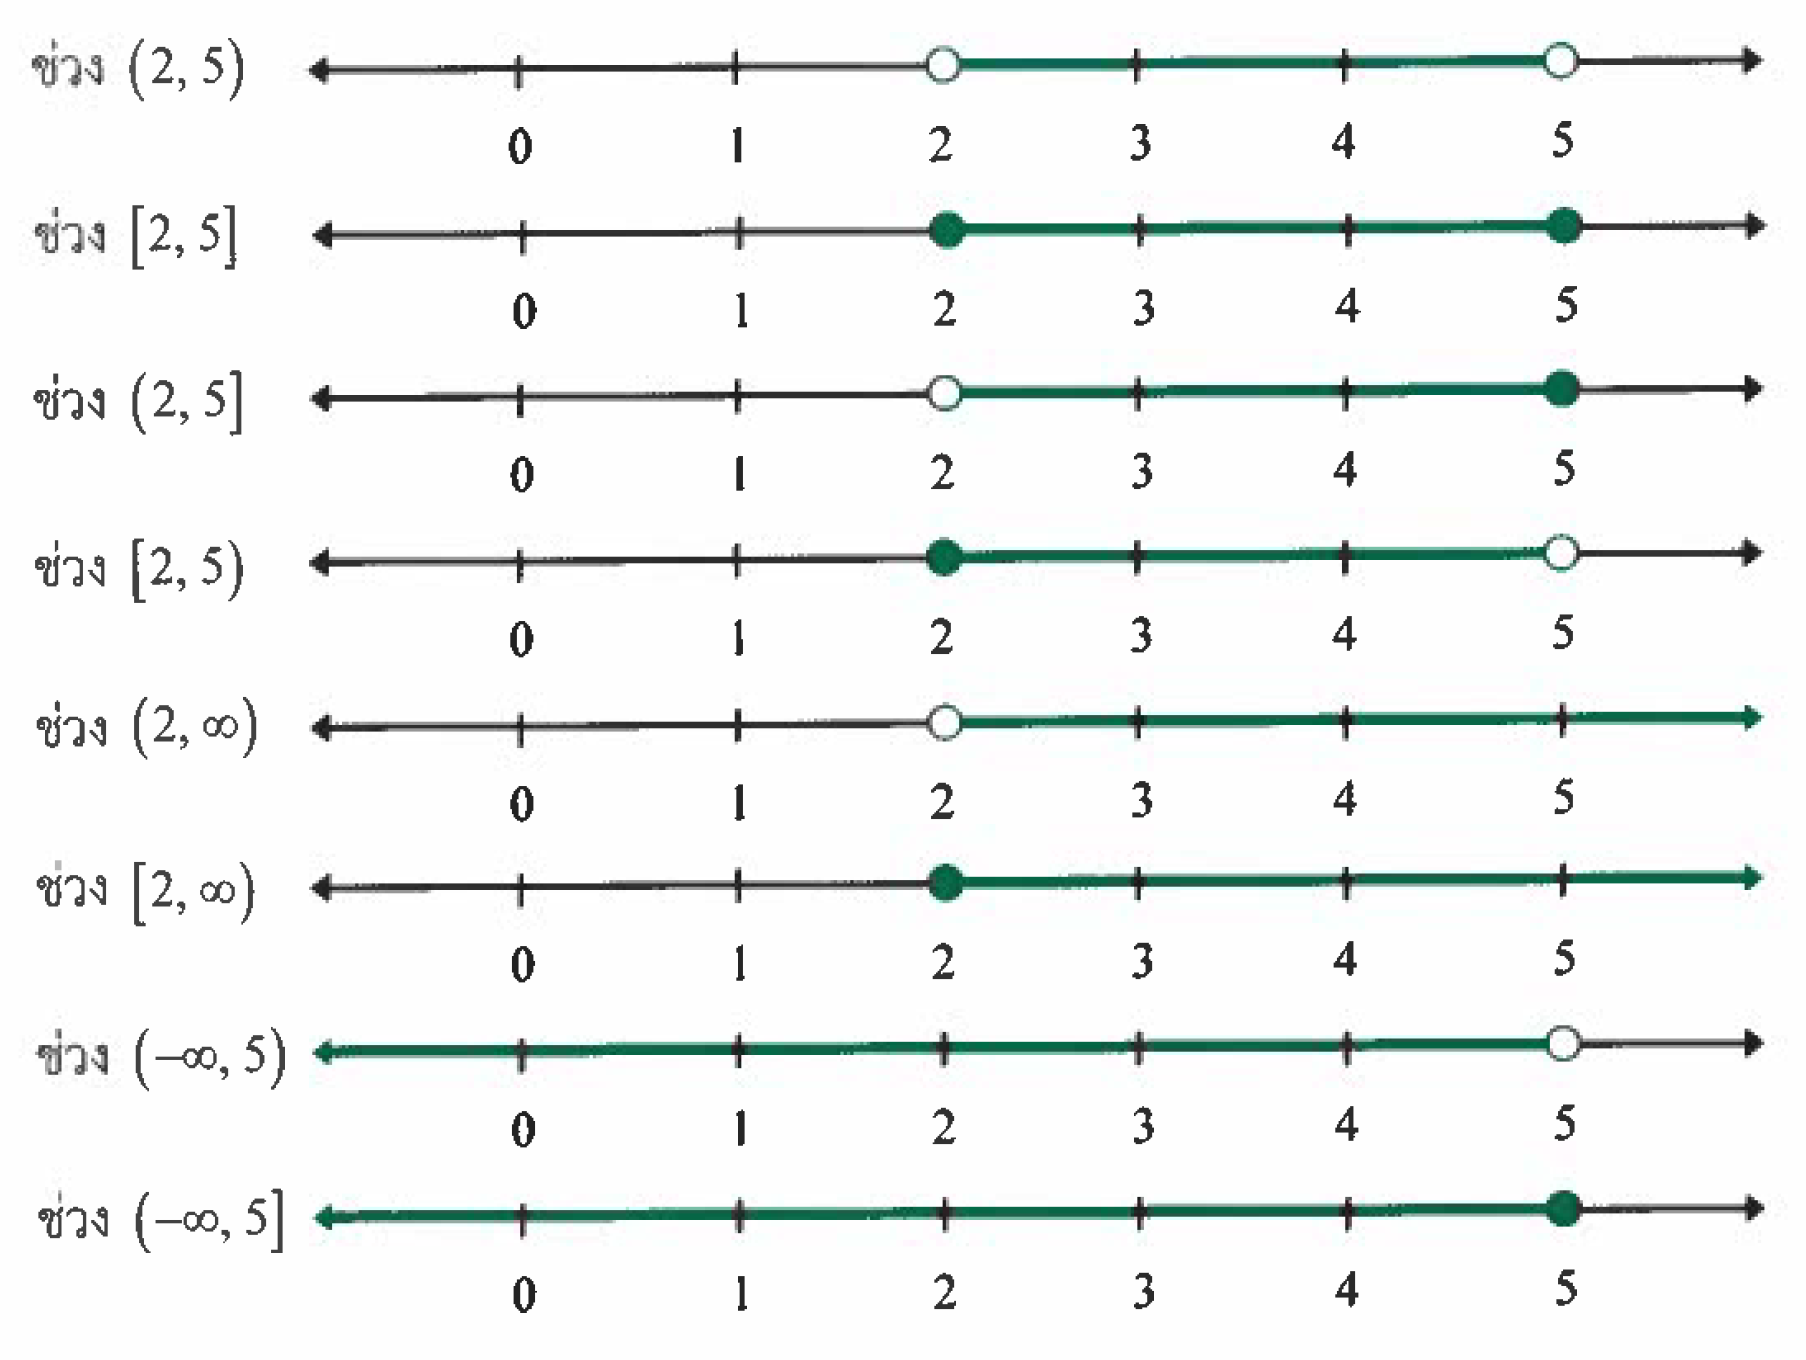
\includegraphics[scale=0.35]{1} 
	\caption{} 
	\label{Figure1} 
\end{figure}

\subsection*{ใบงาน}
\begin{enumerate}[label=\arabic*., leftmargin=*]
	\item จงเขียนช่วงต่อไปนี้ให้อยู่ในรูปของเซตแบบบอกเงื่อนไข พร้อมทั้งแสดงกราฟของช่วงบนเส้นจำนวน
\begin{multicols}{2}
	\begin{enumerate}[label=\theenumi\arabic*), leftmargin=*]
	\item $[-3, 1)$
	\item $(-2, \infty)$
	\item $[4, 7]$
	\item $(-3, 0)$
	\item $(-\infty, -3)$
	\item $[1, \infty)$
	\item $(-1, 4]$
	\item $(-\infty, 1]$
	\item $(-10, -8)$
	\item $[2.5, 4]$
	\item $(-6, 5)$
	\item $\left(\dfrac{1}{2}, \dfrac{3}{2}\right]$
	\item $[0.5, 4.5)$
	\item $[-15, 20]$
	\item $(-\pi, \pi)$
	\item $[-\sqrt{2}, \sqrt{2})$
	\item $(-\infty, \sqrt{3}]$
	\item $(-\infty, -5)$
	\item $\left(\dfrac{5}{2}, \infty\right)$
	\item $[-100, \infty)$
\end{enumerate}
\end{multicols}
\item จงเขียนเซตในข้อต่อไปนี้ในรูปช่วง
	\begin{multicols}{2}
	\begin{enumerate}[label=\theenumi\arabic*), leftmargin=*]
		\everymath{\displaystyle}
		\item $\{x \in \mathbb{R} \mid 2 \leqslant x \leqslant 5\}$
		\item $\{x \in \mathbb{R} \mid -4 < x < 9\}$
		\item $\{x \in \mathbb{R} \mid -10 < x \leqslant 6\}$
		\item $\{x \in \mathbb{R} \mid -7 \leqslant x < -1\}$
		\item $\{x \in \mathbb{R} \mid x \geqslant 5\}$
		\item $\{x \in \mathbb{R} \mid x \leqslant 4\}$
		\item $\{x \in \mathbb{R} \mid x > 12\}$
		\item $\{x \in \mathbb{R} \mid x < -8\}$
		\item $\{x \in \mathbb{R} \mid -\pi \leqslant x \leqslant \pi\}$
		\item $\left\{x \in \mathbb{R} \;\middle|\; x \leqslant \dfrac{\pi}{4}\right\}$
	\end{enumerate}
\end{multicols}

	\item ถ้า $A = (-1, 2)$ และ $B = [0, 4]$ จงเขียนเซตต่อไปนี้ในรูปช่วง
	\begin{multicols}{2}
	\begin{enumerate}[label=\theenumi\arabic*), leftmargin=*]
	\item $A \cup B$
	\item $A \cap B$
	\item $A - B$
	\item $B - A$
	\item $A'$
	\item $B'$
\end{enumerate}
	\end{multicols}
\item กำหนดให้ $A = [-8, 6]$, $B = [-6, 9)$, $C = (-9, 1]$ และ $D = (0, 5)$ จงหาเซตในข้อต่อไปนี้ในรูปช่วง
\begin{multicols}{2}
	\begin{enumerate}[label=\theenumi\arabic*), leftmargin=*]
		\item $A \cap B$
		\item $A \cup B$
		\item $A \cap C$
		\item $A \cup C$
		\item $A \cap D$
		\item $A \cup D$
		\item $B \cap C$
		\item $B \cup C$
		\item $B \cap D$
		\item $B \cup D$
		\item $C \cap D'$
		\item $C \cup D$
		\item $A - B$
		\item $B - A$
		\item $A - C$
		\item $C - A$
		\item $A - D$
		\item $B - D$
		\item $C - D$
		\item $D - B$
	\end{enumerate}
\end{multicols}
\item กำหนดให้ $A = (-\infty, 3]$, $B = [-2, \infty)$, $C = [-4, 4]$ และ $D = (0, 6)$ จงหาเซตในข้อต่อไปนี้ในรูปช่วง
\begin{multicols}{2}
	\begin{enumerate}[label=\theenumi\arabic*), leftmargin=*]
		\item $A \cap B$
		\item $A \cup B$
		\item $A - B$
		\item $A \cap C$
		\item $A \cup C$
		\item $A - C$
		\item $A \cap D$
		\item $A \cup D$
		\item $A - D$
		\item $B \cap C$
		\item $B \cup C$
		\item $B - C$
	\end{enumerate}
\end{multicols}
	\item ถ้า $A = \{x \mid 2 \le x \le 5\}$, $B = \{x \mid -1 < x < 3\}$ และ $C = \{x \mid 1 < x \le 4\}$ จงหาเซตต่อไปนี้
		\begin{multicols}{2}
	\begin{enumerate}[label=\theenumi\arabic*), leftmargin=*]
	\item $B \cup C$
	\item $A \cap C$
	\item $A \cup B \cup C$
	\item $A \cap B \cap C$
	\item $A' \cap B$
	\item $B' \cap C$
	\item $(A \cup B) \cap C$
	\item $(A \cap C) \cup (B \cap C)$
\end{enumerate}
	\end{multicols}
\end{enumerate}
\newpage
\subsection*{อสมการพหุนามตัวแปรเดียว}

อสมการ (inequality) ใช้บ่งถึงประโยคทางคณิตศาสตร์ที่กล่าวถึงการไม่เท่ากัน เช่น $2 > 1$ เป็นอสมการที่เป็นจริง และ $0 < -1$ เป็นอสมการที่เป็นเท็จ 

ในกรณีที่อสมการเป็นประโยคเปิด เช่น 
$$2x < 8, \quad x^2 \geq 0, \quad x^2 + 1 < 0$$
เมื่อนำจำนวนจริงมาแทนตัวแปรในอสมการ จะได้อสมการที่เป็นจริงหรือเท็จ ดังนี้

\vspace{0.5em}
\begin{itemize}[label=\quad, leftmargin=1em, itemsep=0.4em]
	\item เมื่อแทน $x$ ใน $2x < 8$ ด้วยจำนวนจริงที่น้อยกว่า $4$ จะได้อสมการที่เป็นจริง
	\item เมื่อแทน $x$ ใน $x^2 \geq 0$ ด้วยจำนวนจริงใด ๆ จะได้อสมการที่เป็นจริงเสมอ
	\item เมื่อแทน $x$ ใน $x^2 + 1 < 0$ ด้วยจำนวนจริงใด ๆ จะได้อสมการที่เป็นเท็จเสมอ
\end{itemize}

\vspace{0.5em}
เซตคำตอบของอสมการ คือ เซตที่มีสมาชิกเป็นจำนวนจริง ซึ่งเมื่อแทน $x$ ในอสมการด้วยจำนวนจริงเหล่านั้นแล้วได้อสมการที่เป็นจริง

\begin{examplebox}
	จงหาเซตคำตอบของอสมการ 
	$$3x + 5 < x - 7$$
\end{examplebox}
\solution
\newpage

\begin{examplebox}
	จงหาเซตคำตอบของอสมการ 
	$$x^2 - 5x + 6 > 0$$
\end{examplebox}
\solution
\newpage

\begin{examplebox}
	จงหาเซตคำตอบของอสมการ 
	$$x^2 - 2x - 3 \leq 0$$
\end{examplebox}
\solution
\newpage

\begin{examplebox}
	จงหาเซตคำตอบของอสมการ 
	$$\dfrac{1}{x} < \dfrac{1}{2}$$
\end{examplebox}
\solution
\newpage

\begin{examplebox}
	จงหาเซตคำตอบของอสมการ 
	$$\dfrac{x^2 - 12}{x} > -1$$
\end{examplebox}
\solution
\newpage

\begin{examplebox}
	จงหาเซตคำตอบของอสมการ 
	$$\dfrac{x}{x+8} \leq \dfrac{1}{x-1}$$
\end{examplebox}
\solution
\newpage
\subsection*{ใบงาน}
จงหาเซตคำตอบของอสมการต่อไปนี้
\begin{multicols}{2}
	\begin{enumerate}[label=\arabic*., leftmargin=*]
		\item $3 x+1<2 x-1$
		\item $4 y+7>2(y+1)$
		\item $2(3 y-1)>3(y-1)$
		\item $4-(3-x)<3 x-(3-2 x)$
		\item $x^2-x-6 \leq 0$
		\item $2 x^2+7 x+3 \geq 0$
		\item $6 x-x^2 \geq 5$
		\item $2 x<3-x^2$
		\item $x^2+2 x<15$
		\item $3 x^2+2 \geq 7 x$
		\item $x^3-3 x^2 \leq 10 x$
		\item $x^3-x^2-x+1 \geq 0$
		\item $x^3-x>2 x^2-2$
		\item $x\left(x^2+4\right)<5 x^2$
		\item $\dfrac{(x-1)(x+3)}{x-2} \leq 0$
		\item $\dfrac{2 x-3}{(x+2)(x-5)}>0$
		\item $\dfrac{x^2+12}{x}>7$
		\item $\dfrac{x^2+6}{x} \leq 5$
		\item $\dfrac{6}{x-1}>1$
		\item $\dfrac{2 x-4}{x-1}<1$
		\item $\dfrac{6}{x-4} \leq x+1$
		\item $\dfrac{8}{x+2} \geq x$
		\item $\dfrac{5-x}{x^2-3 x+2}<1$
		\item $\dfrac{x+6}{x(x+1)}<6$
		\item $\dfrac{1}{x+1} \geq \dfrac{1}{x+4}$
		\item $\dfrac{1}{x+2} \geq \dfrac{1}{2 x-3}$
		\item $\dfrac{x}{x+2} \geq \dfrac{1}{x}$
		\item $\dfrac{x+1}{2 x-3} \geq \dfrac{1}{x-3}$
		\item $\dfrac{\left(x^2+3 x-10\right)\left(x^2+x-6\right)}{x^2+2 x-15} \geq 0$
		\item $(x-1)^3(x+2)^4>0$
		\item $(x-1)^3(x+2)^4<0$
		\item $(2 x+1)^3(x+1)^5<0$
	\end{enumerate}
\end{multicols}
\newpage
\section{ค่าสัมบูรณ์}

\begin{definitionbox}\label{definition1.6}
	ให้ $a$ เป็นจำนวนจริง \textbf{ค่าสัมบูรณ์ (absolute value)} ของจำนวนจริง $a$ เขียนแทนด้วยสัญลักษณ์ $|a|$ โดยที่
	$$|a| = \begin{cases}
		a & \text{เมื่อ } a \geq 0 \\
		-a & \text{เมื่อ } a < 0
	\end{cases}$$
\end{definitionbox}

\vspace{1em}

\remark
\begin{enumerate}[label=\arabic*., leftmargin=2em, itemsep=0.8em]
	\item จากบทนิยามในกรณีที่ $a < 0$ จะได้ $-a > 0$ แสดงว่า $|a| = -a$ ซึ่งเป็นจำนวนบวก 
	\\
	ดังนั้น สำหรับจำนวนจริง $a$ จะได้ว่า $|a|$ มากกว่าหรือเท่ากับศูนย์ โดยที่
	$$|a| = 0 \quad \text{ก็ต่อเมื่อ} \quad a = 0$$
	
	\item ค่าสัมบูรณ์ของจำนวนจริง $a$ สามารถพิจารณาเชิงเรขาคณิตเป็นระยะทางจากจุดที่แทน $0$ ถึงจุดที่แทน $a$ บนเส้นจำนวน
\end{enumerate}

\begin{theorembox}
ให้ $x$ และ $y$ เป็นจำนวนจริง จะได้ว่า
\begin{enumerate}[label=\arabic*., leftmargin=*]
	\item $|x|=|-x|$
	\item $|x y|=|x||y|$
	\item $\left|\dfrac{x}{y}\right|=\dfrac{|x|}{|y|}$ เมื่อ $y \neq 0$
	\item $|x-y|=|y-x|$
	\item $|x|^2=x^2$
	\item $|x+y| \leq|x|+|y|$
\end{enumerate}
\end{theorembox}

\newpage
\begin{examplebox}
	ให้ $x$ เป็นจำนวนจริง จงแสดงว่า 
	\[
	|x| = |-x|
	\]
\end{examplebox}

\proof

\case เมื่อ $x > 0$

จากบทนิยาม จะได้
\[
|x| = x
\]

และเมื่อ $x > 0$ จะได้ว่า $-x < 0$ จากบทนิยามของค่าสัมบูรณ์ในกรณีค่าติดลบ จึงได้ว่า

\[
|-x| = -(-x) = x
\]

ดังนั้น ในกรณีนี้จะได้ $|x| = |-x|$

\medskip

\case เมื่อ $x = 0$

จากบทนิยาม จะได้

\[
|x| = 0
\quad \text{และ} \quad
|-x| = |-0| = 0
\]

ดังนั้น ในกรณีนี้จะได้ $|x| = |-x|$

\medskip

\case เมื่อ $x < 0$

จากบทนิยาม จะได้

\[
|x| = -x
\]

และเมื่อ $x < 0$ จะได้ว่า $-x > 0$ จากบทนิยามของค่าสัมบูรณ์ในกรณีค่ามากกว่าหรือเท่ากับศูนย์ จึงได้ว่า

\[
|-x| = -x
\]

ดังนั้น ในกรณีนี้จะได้ $|x| = |-x|$

\medskip

จากทั้งสามกรณี สรุปได้ว่า สำหรับทุกจำนวนจริง $x$ จะได้ว่า

\[
|x| = |-x| \quad \text{เสมอ}
\]

\begin{examplebox}
ให้ $x$ และ $y$ เป็นจำนวนจริง จงแสดงว่า 
	\[|x-y|=|y-x|\]	
\end{examplebox}
\proof
$$
\begin{aligned}
	|x-y| & =|-(x-y)| \\
	& =|y-x|
\end{aligned}
$$
\newpage

\begin{remarkbox}
	สำหรับจำนวนจริง $a$ และ $b$ ค่าสัมบูรณ์ของ $a - b$ สามารถพิจารณาเชิงเรขาคณิตเป็นระยะทางจากจุดที่แทน $a$ ถึงจุดที่แทน $b$ บนเส้นจำนวน (นั่นคือ ความยาวของส่วนของเส้นตรงซึ่งมีจุดปลายทั้งสองคือ จุดที่แทน $a$ และจุดที่แทน $b$) เช่น
	
	\begin{figure}[H] 
		\centering 
		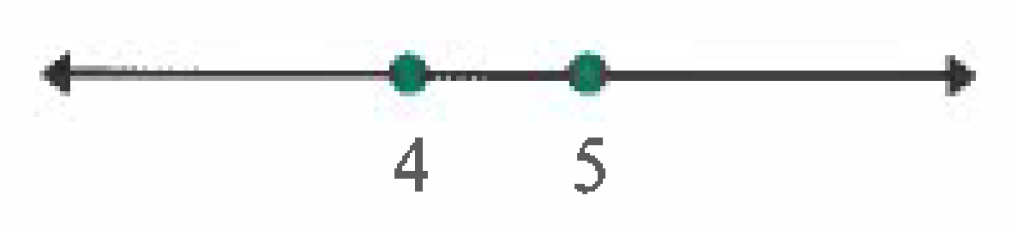
\includegraphics[scale=0.45]{2} 
		\caption{ระยะทางระหว่างจุด $4$ และ $5$ บนเส้นจำนวน} 
		\label{Figure2} 
	\end{figure}
	
	จากรูป \ref{Figure2} ระยะจากจุดที่แทน $4$ ถึงจุดที่แทน $5$ เป็น $1$ หน่วย ซึ่งหาได้จากผลต่างระหว่าง $4$ กับ $5$ เขียนแสดงด้วยค่าสัมบูรณ์ได้เป็น
	$$|5 - 4| \quad \text{หรือ} \quad |4 - 5|$$
	
	\begin{figure}[H] 
		\centering 
		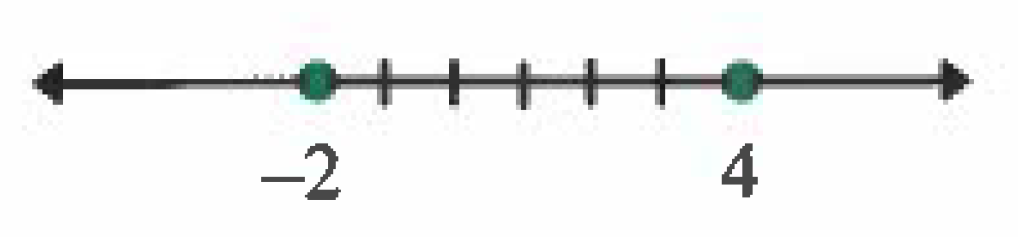
\includegraphics[scale=0.45]{3} 
		\caption{ระยะทางระหว่างจุด $-2$ และ $4$ บนเส้นจำนวน} 
		\label{Figure3} 
	\end{figure}
	
	จากรูป \ref{Figure3} ระยะจากจุดที่แทน $-2$ ถึงจุดที่แทน $4$ เป็น $6$ หน่วย ซึ่งหาได้จากผลต่างระหว่าง $-2$ กับ $4$ เขียนแสดงด้วยค่าสัมบูรณ์ได้เป็น
	$$\Big|4 - (-2)\Big| \quad \text{หรือ} \quad \Big|(-2) - 4\Big|$$
\end{remarkbox}

\newpage
\subsection*{ใบงาน}
\begin{enumerate}[label=\arabic*., leftmargin=*]
	\item จงหาค่าของ
	\begin{enumerate}[label=\theenumi\arabic*), leftmargin=*]
\begin{multicols}{2}
		\item $|-12+8|$
\item $-|25|+|-25|$
\item $|-5(10)|$
\item $-|6|^2$
\item $\left|-\dfrac{28}{6}\right|$
\item $||-2.5|-|3||$
\item $|15-27|$

\item $-\left|-4+9\right|+|7-12|$

\item $\left|\dfrac{-36}{8}\right|$

\item $\left||-7|-|-3|\right|$

\item $-|-4|^2+|3|^2$
\item $|-18+11|$

\item $-|{-8}|+|5-12|$

\item $\left|\dfrac{-45}{12}\right|$

\item $\left||-9|-|4|\right|$

\item $\left||-6+2|-|-5|\right|$
\end{multicols}
	\end{enumerate}
	
	\item ให้ $a$ และ $b$ เป็นจำนวนจริง จงพิจารณาข้อต่อไปนี้ว่าเป็นจริงหรือเท็จ ถ้าเป็นเท็จ ให้ยกตัวอย่างค้าน
	\begin{enumerate}[label=\theenumi\arabic*), leftmargin=*]
		\item $|a+(-b)|=|a|+|-b|$
		\item $|-a|^2=-\left(a^2\right)$
		\item $\left|-\dfrac{a}{b}\right|=\dfrac{|-a|}{|b|}$ เมื่อ $b \neq 0$
		\item $|(-a)(b)|=|-a||b|$
		\item $|-a-b| \leq|-a|-|b|$
		\item ถ้า $a<0$ แล้ว $|a|<a$
	\end{enumerate}
	
	\item จงหาเงื่อนไขของจำนวนจริง $x$ และ $y$ ที่ทำให้
	\begin{enumerate}[label=\theenumi\arabic*), leftmargin=*]
		\item $|x+y|<|x|+|y|$
		\item $|x+y|=|x|+|y|$
	\end{enumerate}
\end{enumerate}

\newpage
\section{สมการและอสมการค่าสัมบูรณ์ของพหุนามตัวแปรเดียว}

เมื่อพิจารณาบนเส้นจำนวน $|x| = a$ หมายถึง จุดที่แทน $x$ อยู่ห่างจากจุดที่แทน $0$ เป็นระยะทาง $a$ หน่วย เมื่อ $a$ เป็นจำนวนจริงบวก เช่น จาก $|x| = 2$ จุดที่แทน $x$ คือ จุดที่อยู่ห่างจากจุดที่แทน $0$ เป็นระยะทาง $2$ หน่วย ซึ่งมีสองจุด ได้แก่ จุดที่แทน $2$ และ $-2$ แสดงบนเส้นจำนวนได้ดังนี้

\vspace{1em}

\begin{figure}[H] 
	\centering 
	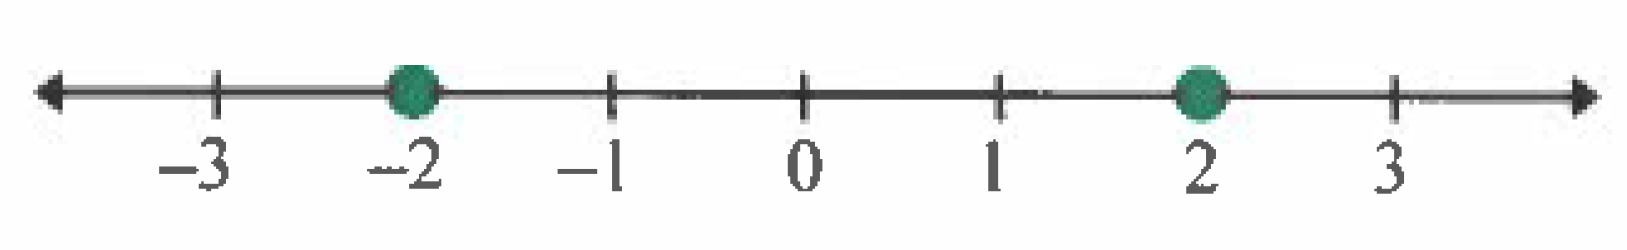
\includegraphics[scale=0.45]{4} 
	\caption{จุดบนเส้นจำนวนที่อยู่ห่างจากจุดแทน $0$ เป็นระยะทาง $2$ หน่วย} 
	\label{Figure4} 
\end{figure}

\vspace{0.5em}
\noindent ดังนั้น เซตคำตอบของสมการ $|x| = 2$ คือ $\{-2, \; 2\}$
\\[0.5em]
สรุปในกรณีทั่วไปได้ตามทฤษฎีบทดังนี้

\vspace{1em}

\begin{theorembox}
	ให้ $a$ เป็นจำนวนจริงบวก
	\\[0.5em]
	เซตคำตอบของสมการ $|x| = a$ คือ $\{-a, \; a\}$
\end{theorembox}

\vspace{1.5em}

\begin{examplebox}
	จงหาเซตคำตอบของสมการ 
	$$|2x + 1| = 5$$
\end{examplebox}
\solution

\newpage

\begin{examplebox}
	จงหาเซตคำตอบของสมการ $|x-1|=2x-3$
\end{examplebox}
\solution

\newpage
\section*{ใบงาน}
จงหาเซตคำตอบของสมการต่อไปนี้
\begin{multicols}{2}
\begin{enumerate}[label=\arabic*., leftmargin=*]
	\item $|5 - 6x| = 0$
	\item $|9x + 6| = 0$
	\item $|1+2x| = 5$
	\item $|2 - 3x| = 10$
	\item $|15 - 8x| = 9$
	\item $|7x + 5| = -2$
	\item $\left|2 x+1\right|=3$
	\item $\left|2 x-5\right|=x+2$
	\item $\left|3 x-2\right|=x-1$
	\item $\left|x\right|=x+2$
	\item $\left|x\right|=3-2 x$
	\item $\left|x^2-x-4\right|=2$
	\item $\left|x-1\right|=\left|2 x+1\right|$
	\item $2\left|x+3\right|=\left|x-2\right|$
	\item $|5x - 2| = |2x + 1|$
	\item $|x| = |4x - 5|$
	\item $|x - 3| = |5 + x|$
	\item $|2 - 5x| = |3x - 1|$
	\item $|x + 1| = |2x - 3|$
	\item $|3x - 2| = |x + 2|$
	\item $|4x - 5| = |3x + 2|$
	\item $|x^2 + 1| = |2x|$
	\item $|x^2 + 3x - 6| = |2x + 6|$
	\item $|2x^2 + 5x - 6| = |x^2 + 4x - 6|$
	\item $|3x + 7| = 5(1+x)$
	\item $|3x - 1| = 2x - 5$
	\item $|x - 3| = 5 + x$
	\item $|4 - x| = x + 4$
	\item $|x| = 6 - 3x$
	\item $|2x + 5| = x$
	\item $|x^2 + 3x - 6| = 2x + 6$
	\item $|2x^2 - 9x - 2| = 2x - 2$
	\item $|x^2 + x| = x^2 - 1$
	\item $|x^2 - 3x - 20| = x^2 + 3x + 2$
\end{enumerate}
\end{multicols}
\newpage

\subsection*{การแก้อสมการในรูปค่าสัมบูรณ์}

พิจารณาอสมการในรูป $|x| < a$ และ $|x| \leq a$ เมื่อ $a$ เป็นจำนวนจริงบวก โดยอาศัยบทนิยามของค่าสัมบูรณ์และใช้เส้นจำนวนเป็นเครื่องช่วย จะได้ตามหลักการ \ref{concept1.8} และ \ref{concept1.9} ดังต่อไปนี้

\begin{conceptbox}\label{concept1.8}
	\begin{itemize}
		\item อสมการ $|x| < a$ หมายถึง จุดที่แทน $x$ อยู่ห่างจากจุดที่แทน $0$ น้อยกว่า $a$ หน่วย
		
		นั่นคือ $|x| < a$ มีความหมายตรงกับอสมการ
		\[
		-a < x \quad \text{และ} \quad x < a
		\]
		ซึ่งเขียนรวมเป็น
		\[
		-a < x < a
		\]
		
		\item อสมการ $|x| \leq a$ หมายถึง จุดที่แทน $x$ อยู่ห่างจากจุดที่แทน $0$ น้อยกว่าหรือเท่ากับ $a$ หน่วย
		
		นั่นคือ $|x| \leq a$ มีความหมายตรงกับอสมการ
		\[
		-a \leq x \quad \text{และ} \quad x \leq a
		\]
		ซึ่งเขียนรวมเป็น
		\[
		-a \leq x \leq a
		\]
	\end{itemize}
\end{conceptbox}

\newpage
\begin{examplebox}
	เมื่อ $a = 2$
	
	จาก $|x| < 2$ จุดที่แทน $x$ แสดงบนเส้นจำนวนได้ดังนี้
	
	\begin{figure}[H]
		\centering
		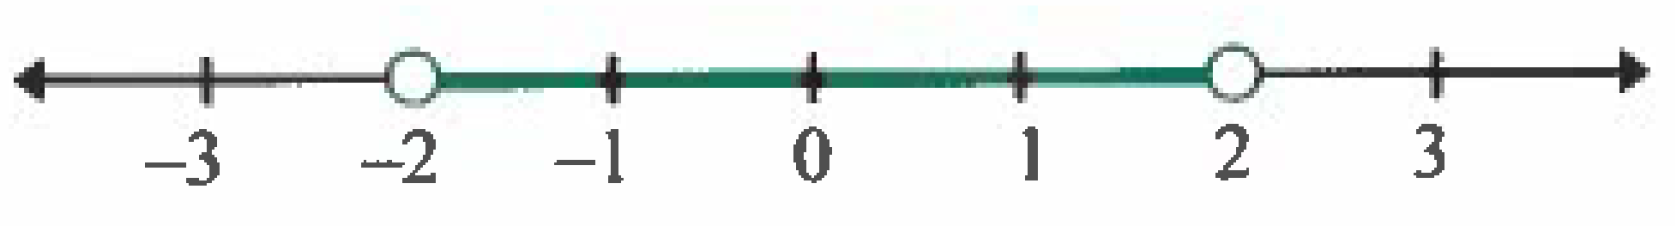
\includegraphics[scale=0.45]{5}
		\caption{กราฟแสดงเซตคำตอบของอสมการ $|x| < 2$}
		\label{Figure5}
	\end{figure}
	
	ซึ่งมีความหมายเหมือนกับ $-2 < x < 2$
	
	ดังนั้น เซตคำตอบของ $|x| < 2$ คือ
	
	\[
	\{x \mid -2 < x < 2\} \quad \text{หรือ} \quad (-2,2)
	\]
	
	\medskip
	
	จาก $|x| \leq 2$ จุดที่แทน $x$ แสดงบนเส้นจำนวนได้ดังนี้
	
	\begin{figure}[H]
		\centering
		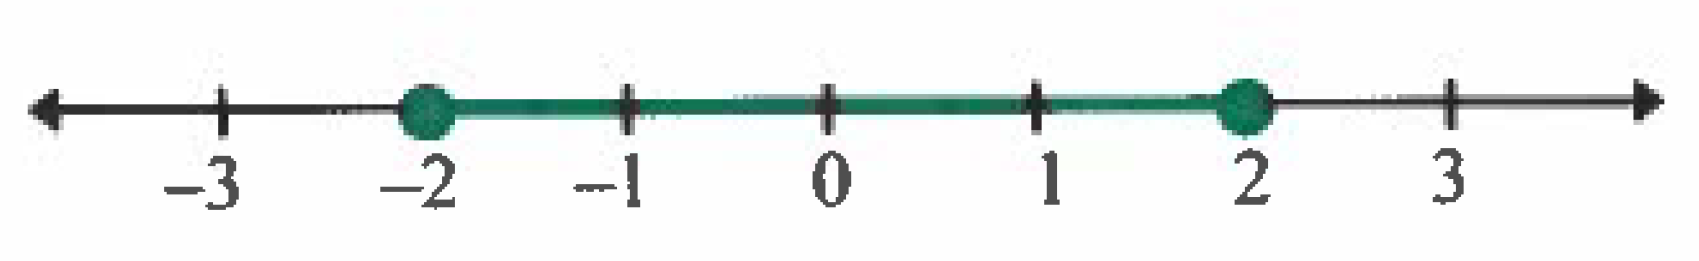
\includegraphics[scale=0.45]{6}
		\caption{กราฟแสดงเซตคำตอบของอสมการ $|x| \leq 2$}
		\label{Figure6}
	\end{figure}
	
	ซึ่งมีความหมายเหมือนกับ $-2 \leq x \leq 2$
	
	ดังนั้น เซตคำตอบของ $|x| \leq 2$ คือ
	
	\[
	\{x \mid -2 \leq x \leq 2\} \quad \text{หรือ} \quad [-2,2]
	\]
\end{examplebox}

\newpage
\begin{conceptbox}\label{concept1.9}
	\begin{itemize}
		\item อสมการ $|x| > a$ หมายถึง จุดที่แทน $x$ อยู่ห่างจากจุดที่แทน $0$ มากกว่า $a$ หน่วย
		
		นั่นคือ $|x| > a$ มีความหมายตรงกับอสมการ
		\[
		x < -a \quad \text{หรือ} \quad x > a
		\]
		
		\item อสมการ $|x| \geq a$ หมายถึง จุดที่แทน $x$ อยู่ห่างจากจุดที่แทน $0$ มากกว่าหรือเท่ากับ $a$ หน่วย
		
		นั่นคือ $|x| \geq a$ มีความหมายตรงกับอสมการ
		\[
		x \leq -a \quad \text{หรือ} \quad x \geq a
		\]
	\end{itemize}
\end{conceptbox}

\newpage

\begin{examplebox}
	เมื่อ $a = 3$
	
	จาก $|x| > 3$ จุดที่แทน $x$ แสดงบนเส้นจำนวนได้ดังนี้
	
	\begin{figure}[H]
		\centering
		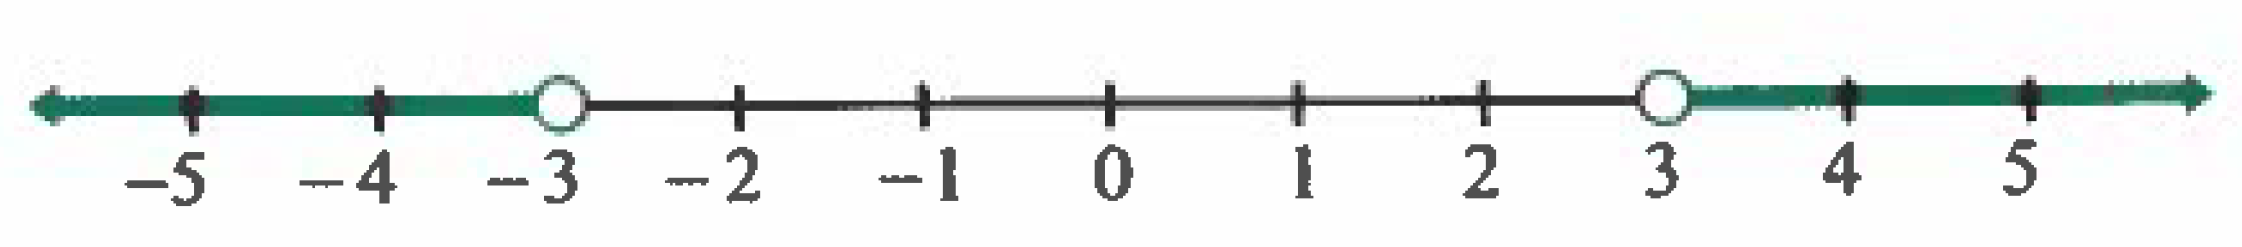
\includegraphics[scale=0.45]{7}
		\caption{กราฟแสดงเซตคำตอบของอสมการ $|x| > 3$}
		\label{Figure7}
	\end{figure}
	
	ซึ่งมีความหมายเหมือนกับ $x < -3$ หรือ $x > 3$
	
	ดังนั้น เซตคำตอบของ $|x| > 3$ คือ
	
	\[
	\{x \mid x < -3 \;\text{หรือ}\; x > 3\}
	\quad \text{หรือ} \quad
	(-\infty,-3)\cup(3,\infty)
	\]
	
	\medskip
	
	จาก $|x| \geq 3$ จุดที่แทน $x$ แสดงบนเส้นจำนวนได้ดังนี้
	
	\begin{figure}[H]
		\centering
		
\includegraphics[scale=0.45]{8}
		\caption{กราฟแสดงเซตคำตอบของอสมการ $|x| \geq 3$}
		\label{Figure8}
	\end{figure}
	
	ซึ่งมีความหมายเหมือนกับ $x \leq -3$ หรือ $x \geq 3$
	
	ดังนั้น เซตคำตอบของ $|x| \geq 3$ คือ
	
	\[
	\{x \mid x \leq -3 \;\text{หรือ}\; x \geq 3\}
	\quad \text{หรือ} \quad
	(-\infty,-3] \cup [3,\infty)
	\]
\end{examplebox}
\newpage
จากที่กล่าวมา สามารถสรุปเป็นทฤษฎีบทได้ดังนี้

\begin{theorembox}
	ให้ $a$ เป็นจำนวนจริงบวก
	\begin{enumerate}
		\item $\left|x\right|<a$ ก็ต่อเมื่อ $-a<x<a$
		\item $\left|x\right| \leq a$ ก็ต่อเมื่อ $-a \leq x \leq a$
		\item $\left|x\right|>a$ ก็ต่อเมื่อ $x<-a$ หรือ $x>a$
		\item $\left|x\right| \geq a$ ก็ต่อเมื่อ $x \leq -a$ หรือ $x \geq a$
	\end{enumerate}
\end{theorembox}

\begin{examplebox}
จงหาเซตคำตอบของอสมการ $|2 x+1|<3$
\end{examplebox}
\solution
\vspace{5cm}

\begin{examplebox}
จงหาเซตคำตอบของอสมการ $\left|\dfrac{x}{2}-3\right| \geq 2$
\end{examplebox}
\solution
\newpage

\begin{examplebox}
	จงหาเซตคำตอบของอสมการ $\left|2x+1\right|< x+5$
\end{examplebox}
\solution
\newpage

\begin{examplebox}
	จงหาเซตคำตอบของอสมการ $\left|\dfrac{1}{2}-\dfrac{x}{2}\right| \leq 1$
\end{examplebox}
\solution
\newpage

\begin{examplebox}
	จงหาเซตคำตอบของอสมการ $2\left|x-1\right|< \left|x+3\right|$
\end{examplebox}
\solution
\vspace{6cm}
\begin{examplebox}
จงหาเซตคำตอบของอสมการ $\left|\dfrac{x-1}{x-2}\right|>2$
\end{examplebox}
\solution
\newpage
\begin{examplebox}
ในแต่ละวัน ถ้าแม่ค้าขายสินค้าได้ $x$ หน่วย แล้วจะมีรายได้ $5 x-15$ บาทต่อวัน โดยเฉลี่ยแม่ค้า มีรายได้วันละ $1,000$ บาท ถ้าต้องการให้รายได้แต่ละวันแตกต่างจากรายได้เฉลี่ยไม่เกิน $50$ บาท แม่ค้าควรขายสินค้าให้ได้วันละกี่หน่วย
\end{examplebox}
\solution

\newpage
\subsection*{ใบงาน}
\begin{enumerate}[label=\arabic*., leftmargin=*]
	\item จงหาเซตคำตอบของอสมการต่อไปนี้
\begin{multicols}{2}
		\begin{enumerate}[label=\theenumi\arabic*), leftmargin=*]
		\item $\left|x-2\right|<1$
		\item $\left|x+3\right|>5$
		\item $\left|3 x+5\right| \geq 4$
		\item $\left|2 x-1\right| \leq 11$
		\item $2\left|x-2\right|>x$
		\item $\left|3 x+4\right| \leq x+2$
		\item $\left|2 x+1\right|<3 x+2$
		\item $\left|x+1\right|>x-3$
		\item $\left|x\right| \geq\left|x-1\right|$
		\item $2\left|x+2\right|<\left|x+3\right|$
		\item $3\left|x-2\right| \leq\left|x+6\right|$
		\item $2\left|2 x-1\right|>3\left|x+1\right|$
		\item $\left|\dfrac{x}{x+4}\right|>2$
		\item $\left|x-\dfrac{4}{x}\right| \leq 3$
		\item $\left|\dfrac{x+1}{x-1}\right|<1$
		\item $\left|\dfrac{x}{x-2}\right|>2$
			\item $|x + 2| > 0$
		\item $|x + 2| \leqslant 0$
		\item $|x + 2| < 0$
		\item $|x + 2| \leqslant 0$
		\item $|x + 3| < 4$
		\item $2|x + 1| \leqslant 8$
		\item $|5 - 2x| > 3$
		\item $3|4 - 2x| > 6$
		\item $\left|\dfrac{x}{2} - 3\right| < 5$
		\item $\left|4 - \dfrac{3x}{2}\right| \geqslant 8$
		\item $|3 x + 4| \leqslant -2$
		\item $|4x - 3| \geqslant -1$
		\item $|5x - 1| < -3$
		\item $|2 - x| > -3$
		\item $|x^2 - x - 1| < 5$
		\item $|x| < 2x$
		\item $|x| \leqslant 1 + 2x$
		\item $|x + 1| > 2x - 3$
		\item $|x - 1| \geqslant x$
		\item $|2x - 3| \leqslant x + 2$
		\item $|x - 2| > 1 - 3x$
		\item $|4x + 5| < -x$
		\item $x + 1 < |2x + 4|$
		\item $|2x - 4| > x + 1$
		\item $|x - 4| \leq 2x + 1$
		\item $|2x - 3| < 3x - 7$
		\item $\left|x^2 - 4\right| \leq \left|x^2 - 2x\right|$
		\item $\left|2x^2 - 5x - 1\right| \leq \left|x^2 - x + 4\right|$
		\item $2\left|\dfrac{x - 1}{x - 5}\right| \leq \left|\dfrac{x - 5}{x - 4}\right|$
		\item $\dfrac{1}{|x| - 2} \geq \dfrac{2}{|x| + 1}$
		\item $\dfrac{|x| + 6}{x + 2} + 1 < \dfrac{|x|}{x - 3}$
		\item $\left|\dfrac{x - 3}{x}\right| \geq \dfrac{x + 5}{x + 2}$
	\end{enumerate}
\end{multicols}

	\item จากการศึกษาของนักดาราศาสตร์พบว่า อุณหภูมิบนพื้นผิวดาวอังคารเป็นไปตามอสมการ $\left|C+84\right| \leq 56$ เมื่อ $C$ แทนอุณหภูมิบนพื้นผิวดาวอังคาร มีหน่วยเป็นองศาเซลเซียส จงหาช่วงของอุณหภูมิบนพื้นผิวของดาวอังคารที่เป็นไปได้จากอสมการนี้
	
	\item ในการทดสอบว่าเหรียญเที่ยงตรงหรือไม่ ทำได้โดยทดลองโยนเหรียญ $100$ ครั้ง แล้วบันทึก จำนวนครั้งที่เหรียญขึ้นหัว กำหนดให้ $x$ เป็นจำนวนครั้งที่เหรียญขึ้นหัว โดยทฤษฎีทางสถิติ กล่าวว่า ถ้าเหรียญที่นำมาทดลองโยนนั้นไม่เที่ยงตรง จะได้ $\left|\dfrac{x-50}{5}\right| \geq 1.645$ จงหา $x$ ที่ทำให้เหรียญไม่เที่ยงตรง
\end{enumerate}


